\documentclass[a4paper,11pt]{article}
\usepackage[utf8]{inputenc}
\usepackage[margin=1in, includefoot,footskip=30pt,]{geometry} %Equivalente a fullpage sem estragar o cabeçalho e rodapé

\usepackage[hidelinks]{hyperref} % Cria hiperligações para imagens e outras referencias
\usepackage{graphicx} %Permite inserir imagens
\usepackage{subcaption} % Permite subfigures

\usepackage{enumitem} % Permite adicionar tab a itemizes
\usepackage{pdfpages} % used to add pdfpages, i.e. the front page
\usepackage{indentfirst}
\usepackage{float}

\usepackage{siunitx}


\usepackage{algorithm}
\usepackage{listings}

\lstset{
%language=py, 
basicstyle=\ttfamily,
numbers=left,
numberstyle=\scriptsize,
stepnumber=1,
numbersep=5pt,
%backgroundcolor=\color{lightlightgray},
tabsize=2,
breaklines=true,
breakatwhitespace=false,
morekeywords={__global__, __device__},
columns=flexible,
keepspaces=true
}


% ----- Definiçoes para as tabelas -----
\usepackage{tabularx}
\newcolumntype{Y}{>{\centering\arraybackslash}X}
\newcolumntype{P}{>{\raggedleft\arraybackslash}X}
\usepackage{booktabs} % alows /toprule and /midrule
\usepackage{multirow}

\usepackage{pdflscape}

\usepackage{lipsum}


\usepackage{xspace}

\newcommand{\admissionId}{\texttt{admission\_id}\xspace}
\newcommand{\patientId}{\texttt{patient\_id}\xspace}
\newcommand{\race}{\texttt{race}\xspace}
\newcommand{\gender}{\texttt{gender}\xspace}
\newcommand{\age}{\texttt{age}\xspace}
\newcommand{\weight}{\texttt{weight}\xspace}
\newcommand{\admissionTypeCode}{\texttt{admission\_type\_code}\xspace}
\newcommand{\dischargeDispositionCode}{\texttt{discharge\_disposition\_code}\xspace}
\newcommand{\admissionSourceCode}{\texttt{admission\_source\_code}\xspace}
\newcommand{\timeInHospital}{\texttt{time\_in\_hospital}\xspace}
\newcommand{\payerCode}{\texttt{payer\_code}\xspace}
\newcommand{\medicalSpecialty}{\texttt{medical\_specialty}\xspace}
\newcommand{\hasProsthesis}{\texttt{has\_prosthesis}\xspace}
\newcommand{\completeVaccinationStatus}{\texttt{complete\_vaccination\_status}\xspace}
\newcommand{\numLabProcedures}{\texttt{num\_lab\_procedures}\xspace}
\newcommand{\numProcedures}{\texttt{num\_procedures}\xspace}
\newcommand{\numMedications}{\texttt{num\_medications}\xspace}
\newcommand{\numberOutpatient}{\texttt{number\_outpatient}\xspace}
\newcommand{\numberEmergency}{\texttt{number\_emergency}\xspace}
\newcommand{\numberInpatient}{\texttt{number\_inpatient}\xspace}
\newcommand{\diagOne}{\texttt{diag\_1}\xspace}
\newcommand{\diagTwo}{\texttt{diag\_2}\xspace}
\newcommand{\diagThree}{\texttt{diag\_3}\xspace}
\newcommand{\numberDiagnoses}{\texttt{number\_diagnoses}\xspace}
\newcommand{\bloodType}{\texttt{blood\_type}\xspace}
\newcommand{\hemoglobinLevel}{\texttt{hemoglobin\_level}\xspace}
\newcommand{\bloodTransfusion}{\texttt{blood\_transfusion}\xspace}
\newcommand{\maxGluSerum}{\texttt{max\_glu\_serum}\xspace}
\newcommand{\AOneCresult}{\texttt{A1Cresult}\xspace}
\newcommand{\diuretics}{\texttt{diuretics}\xspace}
\newcommand{\insulin}{\texttt{insulin}\xspace}
\newcommand{\change}{\texttt{change}\xspace}
\newcommand{\diabetesMed}{\texttt{diabetesMed}\xspace}
\newcommand{\readmitted}{\texttt{readmitted}\xspace}

\begin{document}

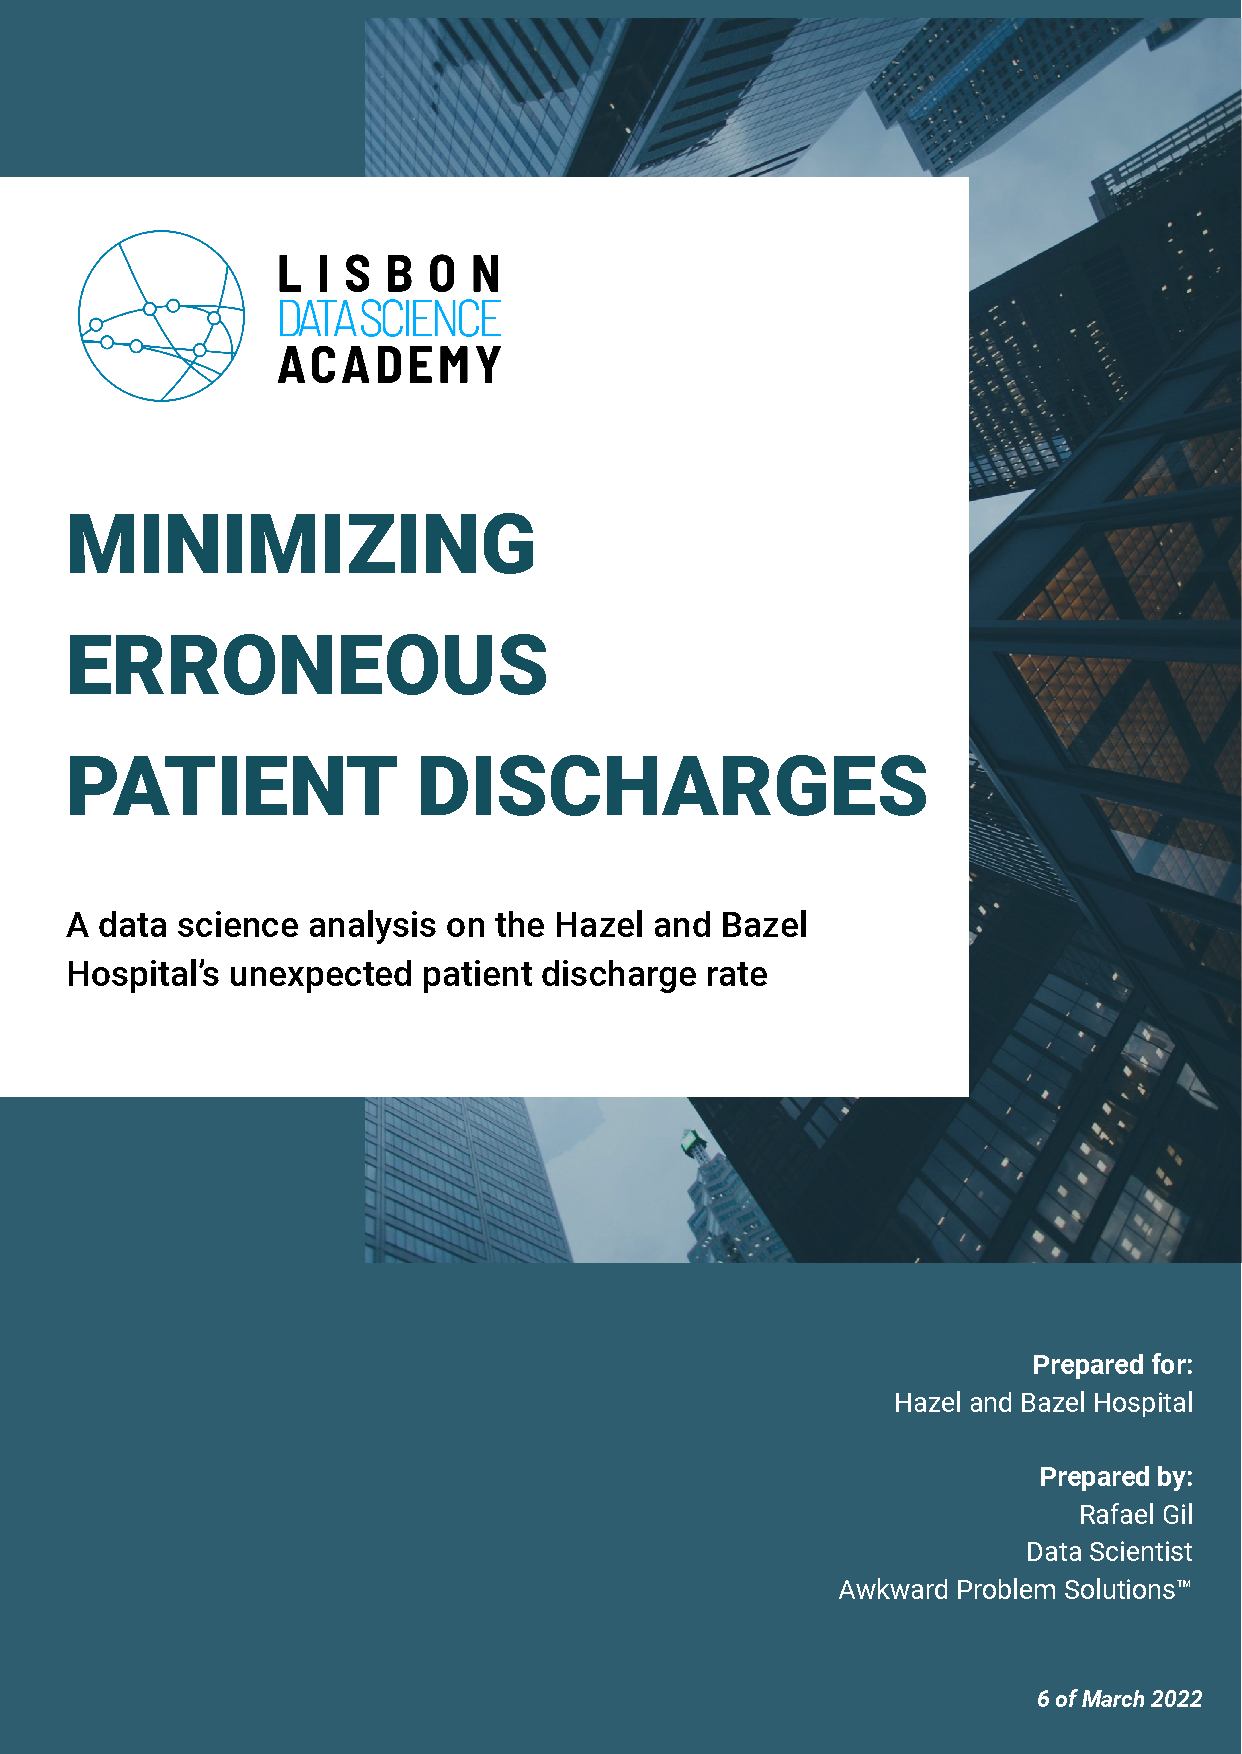
\includepdf[pages={1}]{images/capa.pdf}

\tableofcontents
\newpage


\newpage
\section{Client requirements}
\subsection{Summary}
The Hazel and Bazel hospital, located in Los Angeles, California, is currently under investigation by the Fair Medical Practices Bureau due to suspicions of malpractice. The issue is related to the wrongful medical discharge of patients that return to the hospital within \SI{30}{days} following the medical dismissal.

The hospital hired Awkward Problem Solutions™ to provide insights based on the data analysis of previous medical encounters. The main goal is to identify those patients who are likely to return to the hospital within \SI{30}{days} following a medical discharge.

However, the analysis should also include an investigation into the reasons behind the unexpected patient discharge rate. In particular, if it is a demographic-specific issue or specific to some medical specialties or admission sources. Furthermore, the data analysis must also search for any evidence of discrimination based on gender, ethnicity, age, or insurance status regarding patients discharged from the Hazel and Bazel hospital.

Finally, Awkward Problem Solutions™ should also provide a REST API that integrates with the hospital’s internal system. The API must validate patient discharges based on the medical encounter. In other words, the API should output whether to discharge a patient or not, based on the patient medical encounter information.



\subsection{Requirements clarifications}
\label{sec:requirements_clarifications}

%
\includegraphics[width=0.5\textwidth]{images/to-do.png}

The identified requirements can be divided into two different topics. First, there is the discrimination analysis on sensitive classes. Then, the predictive model deployment and its specifications.

Identifying discrimination, given its nature, is a subjective topic, specially when considering the discrimination on a per medical specialty basis on such a wide range of sensitive classes. There is a high probability of having multiple sub-classes under-represented due to the nature of the medical specialty itself, not discrimination.

Thus, this study will consider discrimination as a  substantial  difference  between a  sensitive  class occurrence, e.g. asian race, in the whole dataset and a readmitted-only subset. The present study considers there is evidence of discrimination if the readmission rate, for a single sensitive class, is higher than \SI{25}{\percent} of the class' overall occurrence.

Regarding, the predictive model, the main goal is to minimize wrongful discharge rate, hence the model should maximize its recall score. However, clarifications revealed that ``at least \SI{50}{\percent} of the patients identified for readmission should actually be sick``. This translates into a minimum of \SI{50}{\percent} precision score. Naturally, this requirement will impact the model recall score, since there is trade-off relationship between precision and recall. Thus, the predictive model should maximize the recall score whilst keeping a precision score above \SI{50}{\percent}.

Finally, in order to ensure no discrimination by the predictive model, it is expected for the readmission rate not to vary more than \SI{10}{\percent} between sub-groups and less than \SI{5}{\percent} between medical specialties. The readmission rate can be measured with the precision score of of each sub-group and medical specialties. Thus, 
the precision score should not to vary more than \SI{10}{\percent} between sub-groups and less than \SI{5}{\percent} between medical specialties.

%This is a very technical question and, as the expert, it should be up to you to make the ultimate decision based on our business requirements: we cannot fail to provide care to a patient that needs it. This means we would like to minimize the number of wrong discharges that would lead patients to return in less than 30 days.

%But we are not made of money so this should not be the only criteria. As a rule of thumb, consider that at least 50% of the patients identified for readmission should actually be sick.

%The wrongful discharge rate, or readmission rate, should not vary more than 10 percentage points between sub-groups, and less than 5 percentage points between medical specialties.



\newpage
\section{Dataset analysis}
\subsection{General analysis}
\label{sec:dataset_general_analysis}
The provided dataset contains information regarding a medical encounters at the hospital. There are \SI{81412}{} rows available, each representing a single medical encounter with \SI{34}{} different variables. 
These variables describe the multiple aspects of a medical encounter, including patient information, diagnosis, and treatments.
A detailed list of the variables included in the dataset is available on table \ref{tab:dtypes}.

Out of the \SI{34}{} variables, \readmitted is our explicit target as it indicates whether or not the patient returned to the hospital within \SI{30}{days} of discharge. However, the number of encounters that resulted in readmission is only \SI{11}{\percent} of the total, making the data at hand highly imbalanced. The remaining variables, described on tables \ref{tab:dtypes} and \ref{tab:dataset_describe} on section \ref{subsection:tech_analysis}, ought to be considered as potential feature candidates.

\subsubsection{Missing values}

The vast majority of the categorical features have at least one or a combination of the following categories: \texttt{?}, \texttt{null}, \texttt{not mapped}, \texttt{not available}, \texttt{unknown/invalid}, \texttt{none}. These values were considered as missing and therefore converted into null before proceeding with the analysis.

Figure \ref{fig:missing_values} lists all the variables available with their non-null percentage and non-null absolute count.

\begin{figure}[htb]
	\centering
	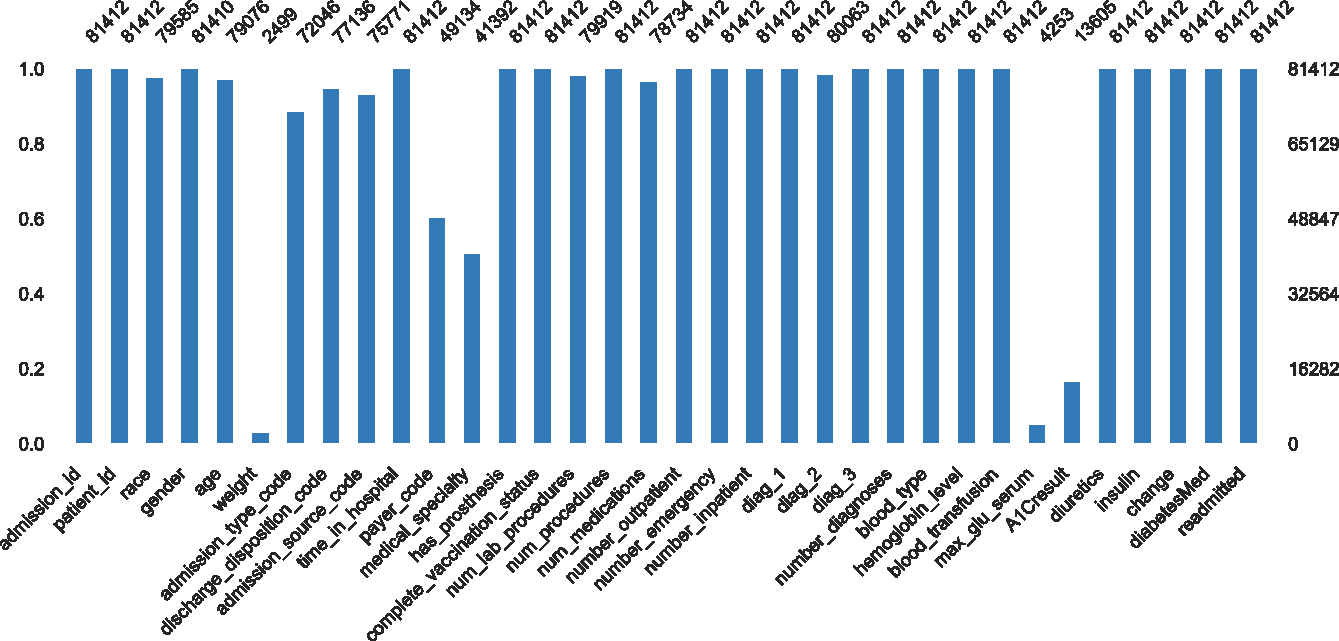
\includegraphics[width=1\textwidth]{images/missing_values.pdf}
	\caption{Medical encounter variables' availability}
	\label{fig:missing_values}
\end{figure}

It is worth noting that \weight, \maxGluSerum, and \AOneCresult are the worst offenders regarding nullability, with \SI{96.9}{\percent}, \SI{94.8}{\percent}, \SI{83.3}{\percent} missing values respectively.  Then, there is \medicalSpecialty, \payerCode, \admissionTypeCode, \admissionSourceCode, with \SI{49.2}{\percent}, \SI{39.6}{\percent}, \SI{11.5}{\percent}, \SI{6.9}{\percent} missing values respectively. There are a few more variables with a residual amount of missing values. 


\subsubsection{Number of unique values}

The following variables have many different categories which will translate into a high dimension feature and may pose a burden on the model convergence:

\paragraph{\medicalSpecialty:}
This variable identifies the medical specialty responsible for discharging the patient. The values available span through a range of \SI{71}{} different medical specialties. However, there are cases where the main specialty is concatenated with a secondary specialty, resulting in a higher category count. For example: '\textit{surgery cardiovascular}', '\textit{surgery cardiovascular/thoracic}', '\textit{surgery colon\&rectal}', '\textit{surgery general}', etc. Those were all merged into the same category ‘\texttt{Surgery}.’ Furthermore, specialties with a count lower than \SI{50}{} were merged into the same ‘\texttt{Others}’ category, reducing the total category count to \SI{24}{} different categories.

\begin{figure}[htb]
	\centering
	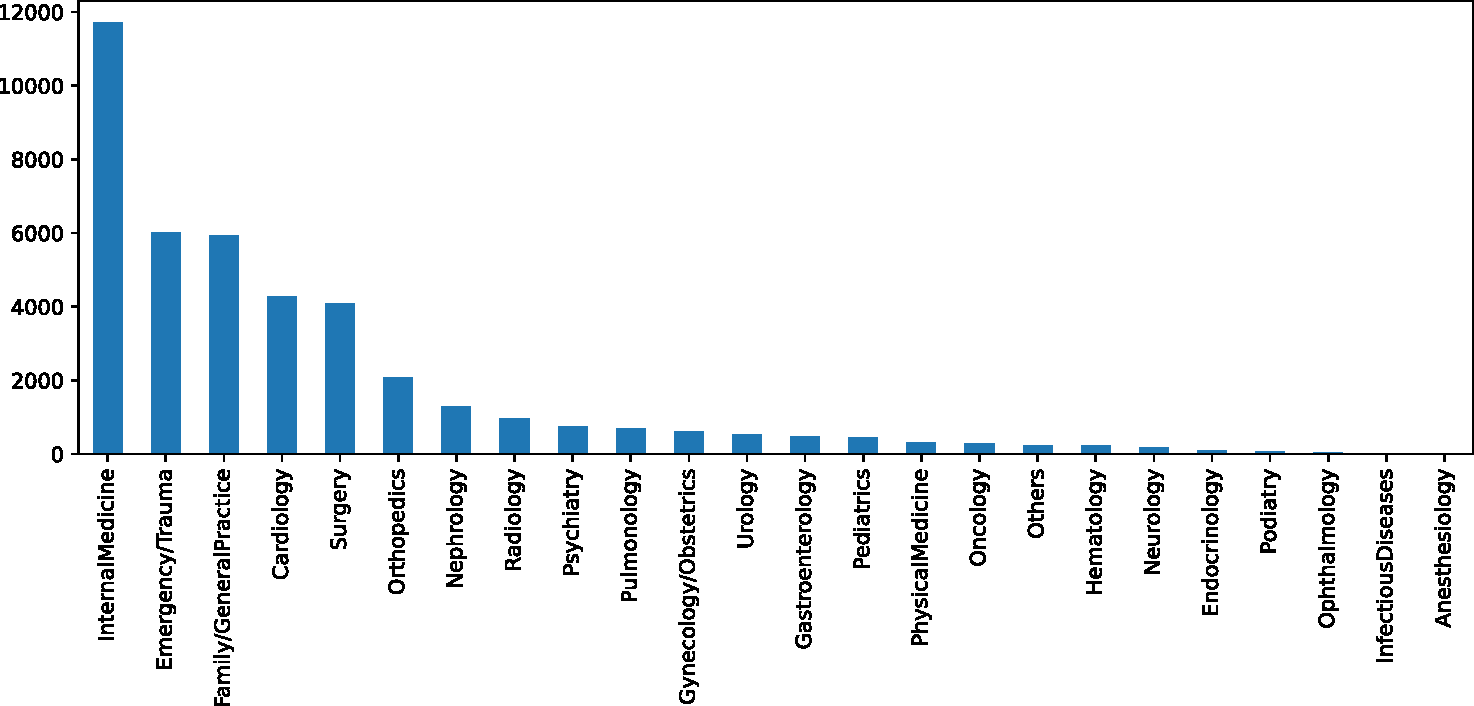
\includegraphics[width=1\textwidth]{images/medical_specialty_cardinality.pdf}
	\caption{Number of medical encounters per medical specialty after processing}
	\label{fig:medical_specialty_cardinality}
\end{figure}


\paragraph{\diagOne, \diagTwo, \diagThree:}
These variables represent the ICD9 codes of the patient's primary, secondary and additional secondary diagnosis. The ICD9 is a list of codes for the International Statistical Classification of Diseases and Related Health Problems. The codes are organized into \SI{18}{} different groups, and, to reduce the feature dimension, each code was converted into its group category. For instance, the codes ranging from $280$ to $289$ all belong to the group \textit{diseases of the blood and blood-forming organs}, thus all these unique values were converted to their group name.

\subsubsection{Correlation}

Figure \ref{fig:correlation} shows the Spearman's correlation matrix of all the variables within the dataset. An initial look, reveals a strong positive correlation between \change, \insulin, and \diabetesMed, with an highlight on \insulin and \diabetesMed. These are all boolean variables with the following meaning:

\begin{itemize}
    \setlength\itemsep{0em} %\itemsep0em
    \item \change indicates if there was a change in diabetic medications;
    \item \insulin indicates whether insulin was prescribed;
    \item \diabetesMed indicates if there was any diabetic medication. prescribed.
\end{itemize}

These variables are all related to diabetes medication and empirically this relationship was expected, given the hospital's focus on patients with diabetes.

Furthermore, it is also worth noting a slight positive correlation between \numMedications and \timeInHospital, as empirically expected.



\begin{figure}[!htb]
	\centering
	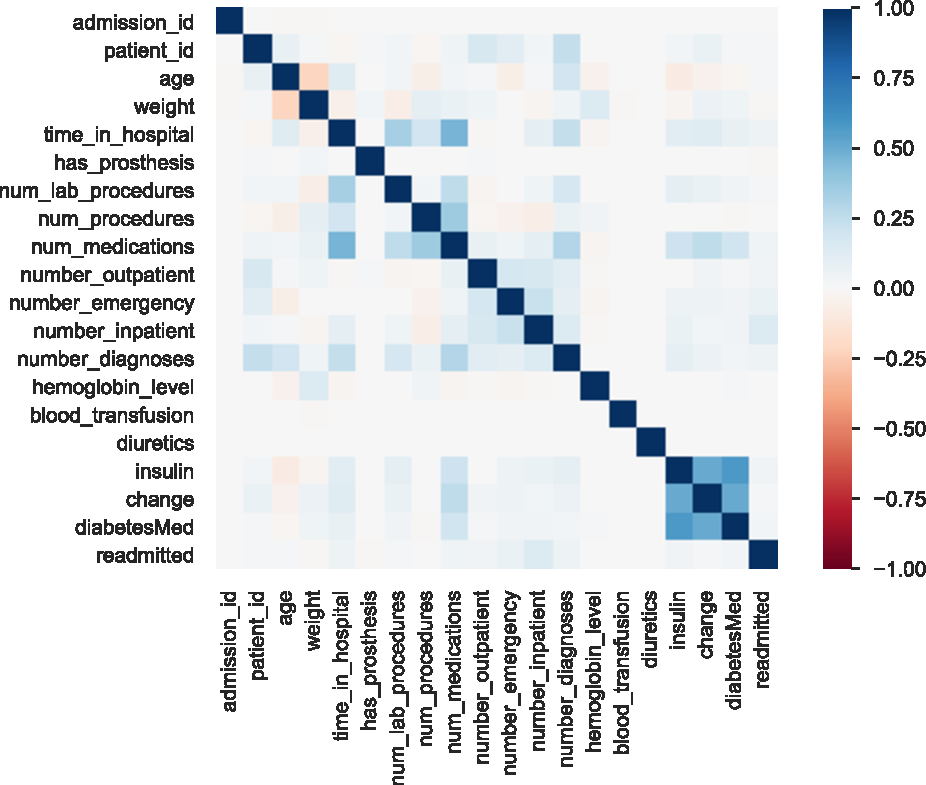
\includegraphics[width=0.7\textwidth]{images/correlation.pdf}
	\caption{Spearman's correlation matrix}
	\label{fig:correlation}
\end{figure}


\subsubsection{Data integrity}
\label{sec:general_analysis_data_integrity}

The provided dataset includes medical encounters of \SI{60069}{} unique patients. Out of those patients, \SI{12647}{}, i.e. \SI{21}{\percent} visited the Hospital more than once. This provides an opportunity to validate the dataset integrity since static patient information should be the same across all its medical encounters. 


The variable \bloodType was chosen to proceed with this analysis. 
\race, and \gender could also be argued as static patient information, but there is a degree of subjectivity to them and there is no chronological information available. %, thus they were not considered.
Hence, the definition of a corrupted medical encounter: A medical encounter is corrupted if there is a second one where the same patient has a different \bloodType.



\begin{figure}[htb]
\centering
\begin{subfigure}{0.32\textwidth}
    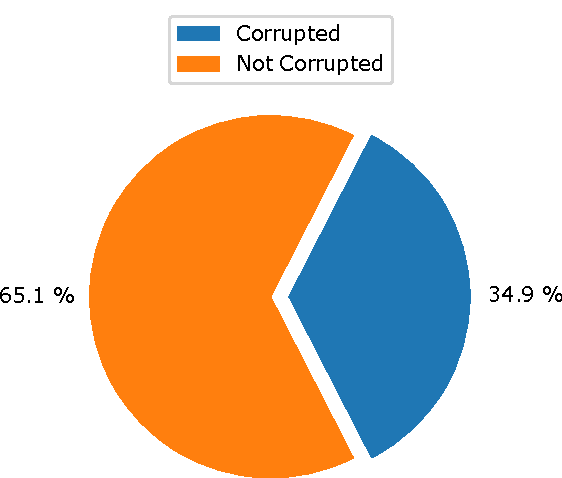
\includegraphics[width=\textwidth]{images/pie_1.pdf}
    \caption{Corrupted medical encounters across the whole dataset}
    \label{fig:duplicated_patients_first}
\end{subfigure}
\hfill
\begin{subfigure}{0.32\textwidth}
    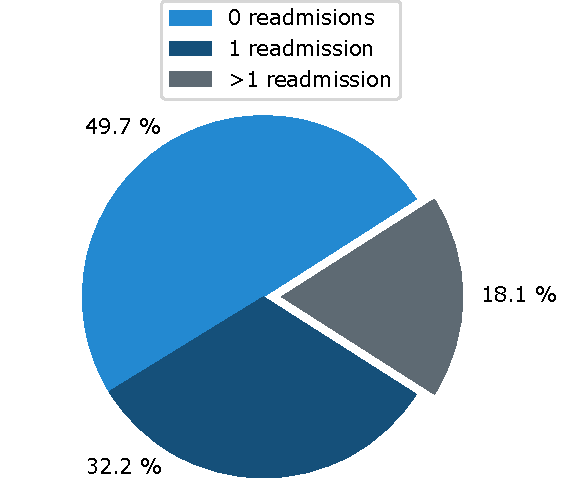
\includegraphics[width=\textwidth]{images/pie_2.pdf}
    \caption{Target/Readmission distribution across the corrupted data}
    \label{fig:duplicated_patients_second}
\end{subfigure}
\hfill
\begin{subfigure}{0.32\textwidth}
    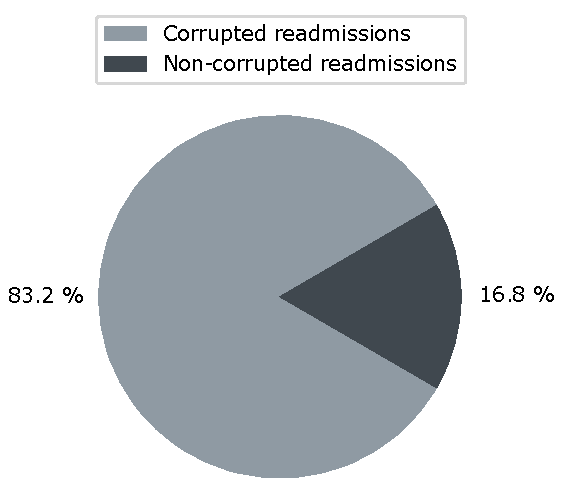
\includegraphics[width=\textwidth]{images/pie_3.pdf}
    \caption{Corrupted distribution on a readmitted-only subset from \ref{fig:duplicated_patients_second}}
    \label{fig:duplicated_patients_third}
\end{subfigure}
        
\caption{Data integrity analysis of based on patients who visited the hospital at least twice}
\label{fig:duplicated_patients}
\end{figure}

Figure \ref{fig:duplicated_patients} summarizes the analysis to the whole dataset based on the corrupted medical encounter definition above. Figure \ref{fig:duplicated_patients_first} shows that \SI{34.9}{\percent} of the data set is corrupted, i.e. each of these medical encounters have at least another one where \bloodType does not match.

Figure \ref{fig:duplicated_patients_second} drills down into the corrupted entries and focus on the target variable: \readmitted. It shows that \SI{49.7}{\percent} of those corrupted medical entries belong to patients that were never readmitted into the hospital. \SI{32.3}{\percent} belongs to patients that were readmitted once. The remaining, \SI{18.1}{\percent} are entries of patients that were readmitted into the hospital at least twice.

Finally, figure \ref{fig:duplicated_patients_third} focus on the \SI{18.1}{\percent} of corrupted medical entries that belong to patients readmitted more than once. 
Assuming that a medical encounter is handled with extra care when a readmission occurs, and knowing that these patients were readmitted more than once, this chart checks if the all their readmitted medical encounters have a matching \bloodType, i.e. if the re-admissions are corrupted when only compared to re-admissions.
It turns out that only \SI{16.8}{\percent} of those medical encounters have the same \bloodType observation for the same patient. 
Of course, these \SI{16.8}{\percent} medical encounters still have at least one non-readmitted observation with a different \bloodType for the same patient, which is why they were considered corrupted in the first place on figure \ref{fig:duplicated_patients_first}.

%It checks if the readmitted medical encounters are still corrupted when only compared to readmitted medical encounters. Concluding that \SI{16.8}{\percent} of the readmitted medical encounters have the same \bloodType observation, even though there is at least one non-readmitted observation with a different \bloodType for the same patient.

%\subsubsection{Available features}

% Small description of the variables
%# Categories convertable to int



\subsection{Business questions analysis}

%\subsubsection{Unexpected discharge rate}

% identify those patients who are likely to return to the hospital within \SI{30}{days} following a medical discharge.

%investigation into the reasons behind the unexpected patient discharge rate.
%demographic-specific issue?
%specific to some medical specialties?
%or admission sources?

%\subsubsection{Discrimination}

%discrimination based on gender, ethnicity, age, or insurance status regarding patients discharged from the Hazel and Bazel hospital.

There were concerns regarding patient discharge discrimination based on age, gender, race, and insurance status on the Hazel and Bazel hospital. To proceed with such analysis,  patient discharge discrimination is hereby defined as substantial difference between a sensitive class occurrence in the whole dataset and a readmitted-only subset.
In other words, there is evidence of discrimination if the occurrence of a sensitive class, e.g. asian race, is substantially higher on re-admissions when compared to the whole hospital's data.

Figure \ref{fig:discrim_global} details a discrimination analysis for the variables age, gender, race, and insurance status. In blue its plotted the occurrence of each sensitive class on the whole dataset, whilst in orange its plotted the occurrence of the same sensitive class across the readmission-only subset.

Empirically, from figure \ref{fig:discrim_global}, there is no evidence of discrimination. There is only a slight issue of over-discharging the \SI{70}{years\ old} age group and under-discharging the \SI{50}{years\ old} age group, even though this is not an alarming discrepancy.
Thus, the Hazel and Bazel hospital as whole does not discriminate on any of the studies variables when discharging patients.

\begin{figure}[htb]
\centering
\begin{subfigure}{0.24\textwidth}
    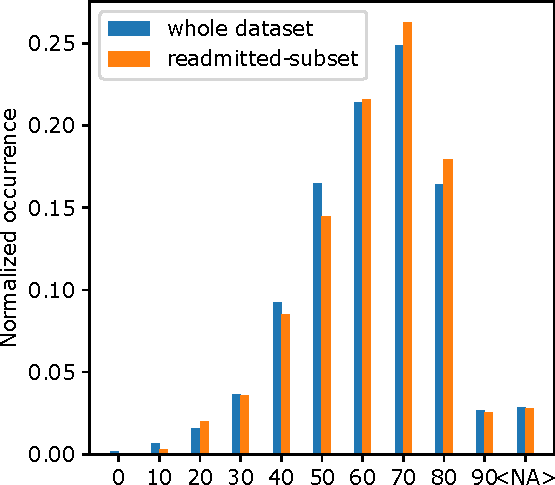
\includegraphics[width=\textwidth]{images/discrim_global_age.pdf}
    \caption{Age}
    \label{fig:discrim_global_age}
\end{subfigure}
\hfill
\begin{subfigure}{0.24\textwidth}
    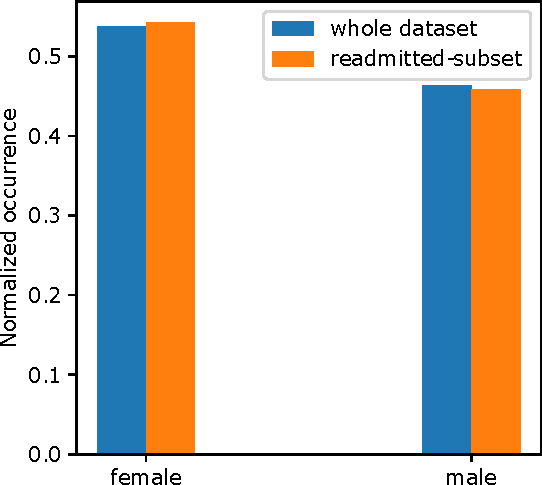
\includegraphics[width=\textwidth]{images/discrim_global_gender.pdf}
    \caption{Gender}
    \label{fig:discrim_global_gender}
\end{subfigure}
\hfill
\begin{subfigure}{0.24\textwidth}
    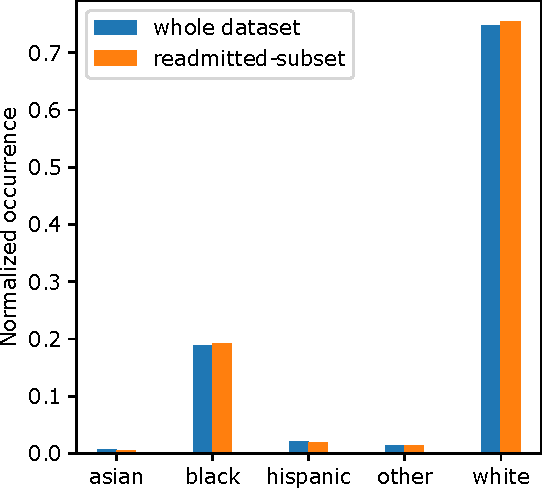
\includegraphics[width=\textwidth]{images/discrim_global_race.pdf}
    \caption{Race}
    \label{fig:discrim_global_race}
\end{subfigure}
\hfill
\begin{subfigure}{0.24\textwidth}
    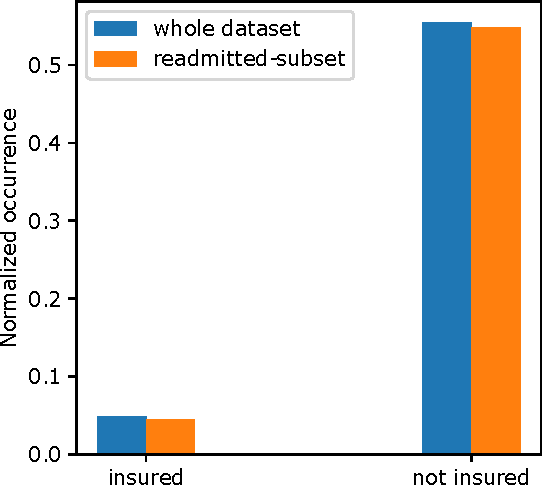
\includegraphics[width=\textwidth]{images/discrim_global_is_insured.pdf}
    \caption{Insurance status}
    \label{fig:discrim_global_is_insured}
\end{subfigure}
\caption{Sensitive classes distribution across the whole dataset and a readmitted-only subset}
\label{fig:discrim_global}
\end{figure}

However, the same analysis can be extended to each medical-specialty, thus revealing discrimination issues on a per-specialty basis. This allows finding out if there are discrimination issues on a single medical specialty that may have been hidden by the remaining medical specialties.

Analogously to the previous analysis, the discharge rate of the sensitive classes within a medical specialty was compared to the medical specialty's overall discharge rate. This study however, yielded different results. First, it was established a threshold of \SI{25}{\percent} between the sensitive class occurrence and its discharge rate within a medical specialty. 
Assuming this threshold, there are many discrimination issues on different medical specialties.
However, it is worth noting that the business requirements mention a lower \SI{10}{\percent} threshold. Naturally, this results in higher discrimination occurrences, which shifts the focus from the worst offenders on this data analysis. Nonetheless, the processed data available here is normalized, making it agnostic to the threshold itself. Thus, this decision only impacts the highlighted medical specialties. 


\begin{figure}[!htb]
	\centering
	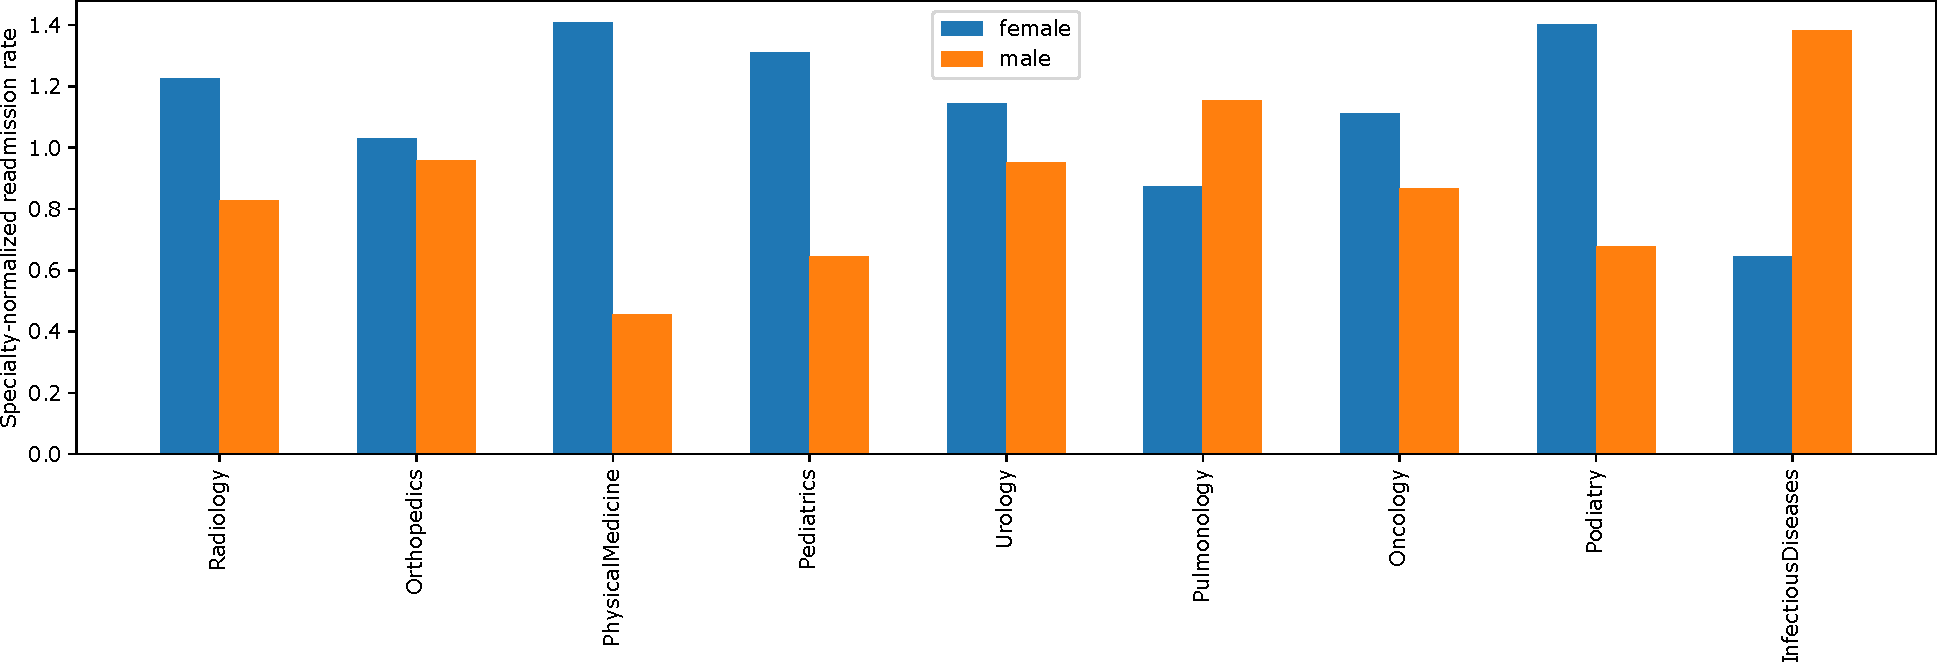
\includegraphics[width=1\textwidth]{images/descrimination_histogram_gender.pdf}
	\caption{Gender discrimination analysis per medical specialty}
	\label{fig:discrimination_histogram_gender}
\end{figure}

Figure \ref{fig:discrimination_histogram_gender} summarizes the results of the per-specialty discrimination on the gender sensitive variable. The graph is built based on the data from table \ref{tab:discrimination_analysis}, available on section \ref{subsection:business_tech_analysis}, along with the other variable's discrimination analysis. It shows, for instance, that the \textit{Physical Medicine} medical specialty has readmission rate of female patients almost \SI{40}{\percent} above the specialty's readmission rate. Meaning \textit{Physical Medicine} is discriminating against women by early discharging female patients.
A similar graphic is available on figures \ref{fig:discrimination_histogram_age}, \ref{fig:discrimination_histogram_race}, and \ref{fig:discrimination_histogram_is_insured}, on section \ref{sec:business_questions_tech}, regarding the remaining sensitive classes.

Given the analysis, and the discrimination definition above, every medical specialty, with the exception of \textit{Internal Medicine} and \textit{Family/General Practice}, is discriminating against at least one sensitive class.

\subsection{Conclusions and Recommendations}


Discrimination data seems alarming, but it does not mean there is structural discrimination on every specialization. For instance, \textit{Pediatrics} shows a strong discrimination for age groups ranging from \SI{60}{years\ old} to \SI{80}{years\ old}, but this actually makes sense given the specialty's focus on lower age groups. Furthermore, medical specialties with lower registered medical encounters, such as \textit{Endocrinology} — check its medical encounter count on figure \ref{fig:medical_specialty_cardinality} — have a higher probability of triggering precisely due to the low amount of medical encounters. This is enhanced by the fact that \textit{Internal Medicine} and \textit{Family/General Practice}, the non-discriminating medical specialties, are among the specialties with the most amount of medical encounters.

Also, the readmission discrimination analysis could be replicated for other variables such as \timeInHospital, \numLabProcedures, \numberDiagnoses, and \change. This would allow identifying if the hospital is also discriminating on the patient's procedures and consequently strengthen the present analysis.

Finally, it is advised that the hospital focus on the specialties with the most medical encounters, that are indeed discriminating. For instance, the hospital is advised to verify the reasons behind \textit{Emergency/Trauma} discrimination against young adults, the reasons behind the \textit{Cardiology} discrimination against \SI{10}{year \ olds}, or the reasons behind the \textit{Orthopedics} discrimination against old patients and hispanics. Refer to table \ref{tab:discrimination_analysis} for further details on the discrimination analysis.


\newpage
\section{Modelling}
\subsection{Model expected outcomes overview}

% threshold, precision, recall, f1_score
%RandomForestClassifier: 
%* train: (0.85, 1.0, 0.5208046293744834, 0.7084148727984344) 0.6849066859938395
%* test: (0.6, 0.7942206654991243, 0.5, 0.7084148727984344) 0.6136671177266576

%LogisticRegression:
%* train: (0.64, 0.8352428964252979, 0.5022044640396803, 0.7068466730954677), 0.6272586473928755
%* test: (0.61, 0.79701230228471, 0.5, 0.7068466730954677), 0.6144986449864499

%Stochastic gradient descent:
%* train: (0.64, 0.8209684584629053, 0.5092311931661615, 0.6967310904318779) 0.6285714285714286
%* test: (0.61, 0.7905982905982906, 0.5099228224917309, 0.6967310904318779) 0.6199731903485254

%Gradient boosting classifier:
%train: (0.65, 0.8324654743038261, 0.5066133921190411, 0.7111869363880088) 0.6298929336188437
%test: (0.62, 0.7980684811237928, 0.5011025358324146, 0.7111869363880088) 0.6156451066711819



The final classifier is able to identify a medical encounter that may result in a patient readmission within \SI{30}{days}. According to the tests, it has an accuracy of \SI{68}{\percent} and a recall of \SI{79}{\percent}. \SI{68}{\percent} accuracy means the model correctly identifies slightly more than \SI{2}{} out of \SI{3}{} medical encounters as a readmission or no-readmission, hence. On the other hand, \SI{79}{\percent} recall means that out of the medical encounters that are readmitted, the model correctly identifies \SI{79}{\percent} as readmissions. Recall is the measure of how good the model is at minimizing the erroneous patient discharge rate.

Recall, as mentioned, is the ability of the model to find all the medical encounters that will be readmitted, whilst precision is its ability not to mark as a potential readmission the medical encounters that won't be readmitted. 
Naturally, both these metrics have a trade-off relationship that is 
%this requirement slightly impacts the model overall precision.
illustrated by figure \ref{fig:precision_recall_evolution}.

The provided dataset, as discussed in section \ref{sec:dataset_general_analysis}, is highly imbalanced meaning the amount of medical encounters that led to a readmission is a small fraction of the total dataset. The predictive models are highly sensitive to this issue and may not generalize as expected, 
%However, even though the tests were made on data that the model did not use during training, it is expected for the 
resulting in real accuracy lower than the \SI{68}{\percent} mentioned above. 
%, due to the smaller training and testing set. 
This accuracy has into account the requirement that at least \SI{50}{\percent} of the patients identified  for  readmission are actually sick, whilst minimizing the number of erroneous medical discharges, i.e. maximizing recall whilst keeping precision above \SI{50}{\percent}. 

Furthermore, there are issues regarding the discrimination requirements and the reason is twofold. On one hand, there are few, i.e less than \SI{100}{}, medical encounters for each sensitive class, e.g asian race, hispanic race, etc. One the other hand, there is a wide range of sensitive classes, meaning there are a lot of different races and age groups. On top of that, there is also a wide range of medical specialties, further distributing the already low amount of classes throughout the medical specialties. 
Nonetheless, in an effort to reduce discrimination, the model was trained without access to these variables at the cost of a slightly lower performance.

As discussed in detail on section \ref{sec:expected_outcomes}, the model is most sensitive to the \numberInpatient variable, i.e. the number of inpatient visits of the patient in the year preceding the encounter.


\subsection{Model specifications}

In order to overcome the imbalanced dataset issue, it was under-sampled, since there there are over \SI{80000}{records} available. First, the corrupted non-readmitted medical encounters, identified in figure \ref{fig:duplicated_patients_first} of the dataset general analysis from section \ref{sec:general_analysis_data_integrity}, were removed.
Afterwards, a set of non-readmitted medical encounters was removed randomly until the target variable was finally balanced.

A different approach could be taken to reduce the amount of randomly removed samples. For instance dropping some specific \dischargeDispositionCode that may not represent a discharge from a medical facility. Nonetheless, this approach required further confirmation by the client.

Having the under-sampled dataset, the data was further divided into train and test data using a \SI{80}{\percent}/\SI{20}{\percent} split, respectively. but keeping in mind that the target class should be evenly distributed among the two groups. Also, the target variable was extracted from each of the groups.

After this, the data is ready for the pipeline. The main focus was building a robust predictive model that could handle all kinds of input data, so a multi-step pre-processing was applied before the predictive model itself:

\begin{enumerate}
    \item \textsc{Pre-processing transformer - Convert input into valid data}
    
    This step is responsible for converting raw data into the model's expected values and categories. The variables' types are checked and converted to an expected value if possible or \texttt{NaN} otherwise. Also, the categories are grouped and parsed at this staged to avoid duplicated and similar classes.
    There are also variables that are converted from categorical into numerical at this stage, such as \age, \weight, \hemoglobinLevel, \maxGluSerum, and \AOneCresult.
    
    \item \textsc{Column-dropper transformer}
    
    This step is used as a handy and centralized location for column dropping. It was specially useful during the model's testing. Here the following columns are removed: 
    
    \begin{itemize}
        \item \admissionId and \patientId, as mentioned in section \ref{sec:dataset_general_analysis}, these are identifiers and have no predictive value;
        
        \item \weight and \maxGluSerum, since both have over \SI{90}{\percent} of missing values;
        
        \item \insulin, because it is highly correlated with \change and \diabetesMed
        
        \item \age, \gender, \race, ad \medicalSpecialty, these are the sensitive variables, and they were removed and added interchangeably in order to evaluate their impact on the model's final discrimination.
    \end{itemize}
     
    \item \textsc{Value imputer}
    
    This step is useful to impute data that the first step could not. 
    Categories that had missing values are filled with an extra \texttt{unknown} category. The remaining categorical and boolean variables with missing data are filled with the most common category. Numeric variables missing data, on the other hand, are imputed with their variable's mean.
    
    \item \textsc{One-hot Encoder / Standard Scaler}
    
    On one hand, the one-hot encoder applies only to the categorical values and its goal is to convert those variables into numerical that the model can consume. On the other hand, the Standard Scaler is used to scale the numerical features exclusively.
    
    
    \item \textsc{Classifier}
    
    Finally, the model is executed at the last stage of the pipeline. The chosen model, as discussed in section \ref{sec:model_alternatives}, is the \textit{Gradient Boosting Classifier} with a maximum depth of $3$, a total of \SI{25}{estimators}, and a learning rate of \SI{10}{\percent}. 
    These hyper-parameters were chosen after running a grid search that provided the best F1 score.
    %\textit{Random Forest Classifier}
    
\end{enumerate}

After training the pipeline, it should calculate the probability of the two studied classes: \texttt{True} meaning the patient is expected to be readmitted, \texttt{False} meaning the patient is not expected to be readmitted. The last final step is to use this information to find the best deciding threshold that maximizes recall whilst keeping precision above \SI{50}{\percent}, based on the test set predicted probabilities. The threshold that best fits the current model is \SI{38}{\percent}. Figure \ref{fig:precision_recall_evolution} graphs the evolution of recall, precision, and accuracy when using different thresholds.

\subsection{Analysis of expected outcomes based on training set}
\label{sec:expected_outcomes}

The evaluated models are all prune to over fitting, meaning they easily memorize the training data and fail to generalize the problem. %This is clear when the training accuracy is substantially higher than the test precision.
To handle this issue the number of estimators and the model's max depth were reduced, thus forcing the model to focus on the most important variables. 

Figure \ref{fig:feature_importance} plots the feature importance of the final model. As discussed the most important feature is the \numberInpatient, with over \SI{30}{\percent} importance. Followed by \numberOutpatient, \numberEmergency, and \numberDiagnoses.

The model has an recall of \SI{79}{\percent} whilst keeping a precision above \SI{65}{\percent}. In other words, the model correctly identifies \SI{79}{\percent} of the medical encounters as readmissions out of those that are actually readmitted, whilst making sure that at least \SI{65}{\percent} of the readmitted are actually sick.

This is achieved with a threshold of \SI{38}{\percent}, meaning the model has to output a probability of readmission higher than \SI{38}{\percent} for the model to consider it as a readmission. This threshold is the one that maximizes recall keeping precision above \SI{65}{\percent}.


\begin{figure}[!htb]
	\centering
	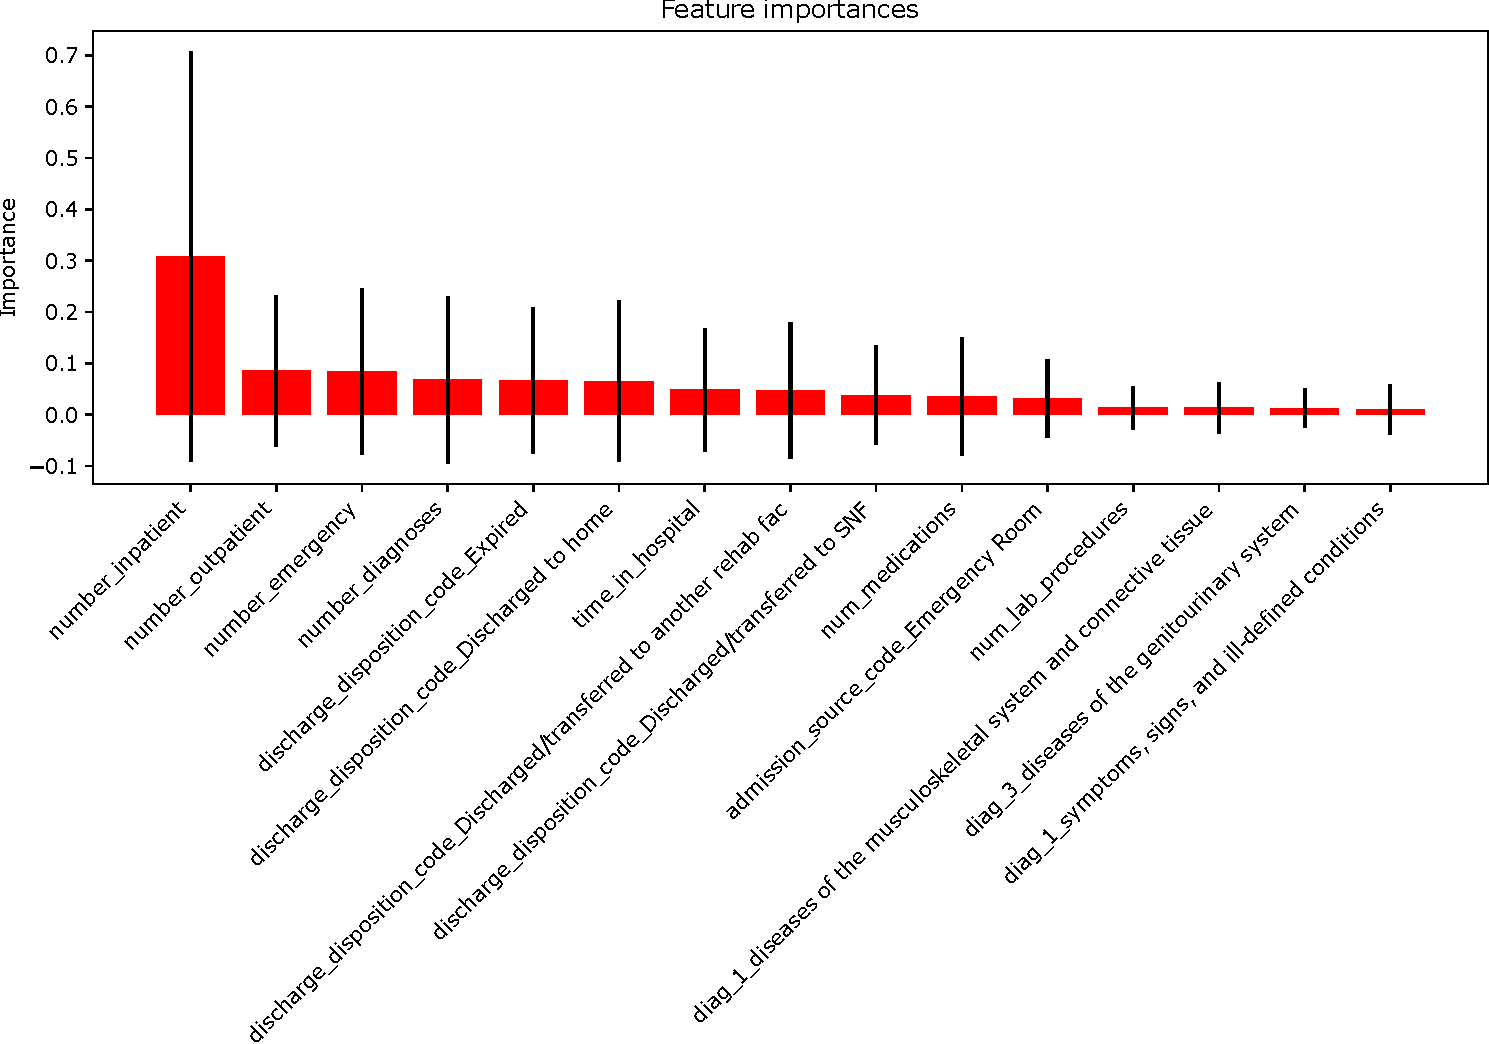
\includegraphics[width=1\textwidth]{images/feature_importance.pdf}
	\caption{Final model's feature importance}
	\label{fig:feature_importance}
\end{figure}


Regarding discrimination, the business requirements state that the model should keep the readmission rate variance below \SI{10}{\percent} between sub-groups and below \SI{5}{\percent} between medical specialties. As mentioned, the readmission rate can be measured through the precision score of each sub-group and medical specialties.
Figure \ref{fig:discrim_req_sensitive} plots the model's precision score for the different sensitive classes, whilst figure \ref{fig:discrim_req_medical_specialty} plots the model's precision scores for the different medical specialties.

The results do not meet all criteria mainly due to the low amount of observations on the test set, and consequently on each of the sensitive classes, due to the undersampling.  
Two sub-groups meet the criteria: gender, and insurance status with precision scores ranging a maximum of \SI{4.86}{\percent} and \SI{4.73}{\percent}, respectively. However, the criteria is not met for age, and race with with precision scores ranging a maximum of \SI{36.66}{\percent} and \SI{19.05}{\percent}, respectively. Note that age and race are sensitive variables with a higher number of categories, and consequently each category has a lower amount of observations. A low amount of observations produces spikes on the precision score that render this discrimination requirement difficult to overcome.
The medical specialty requirement also did not meet the requirement with a precision variance of \SI{47,29}{\percent}. There are even more medical specialties than age and race categories, thus the same rationale applies.
%Dropping the columns related to sensitive classes slightly improved the overall discrimination producing the mentioned results, even though the requirements were not met for all the medical specialties.

The sensitive classes were removed from the training data in an effort to reduce explicit discrimination. Thus, the model has no access to those variables when predicting a result. Unfortunately, this does not mean there won't be discrimination. 
Nonetheless, higher volumes of data may reveal the discrimination is lower than the results now reveal.

%age - 0.3666666666666667
%race - 0.19047619047619047
%gender - 0.04862579281183932
%is_insured - 0.04737160349193148
%medical_specialty - 0.472972972972973


% Overfitting
% Tradeoffs com discrimination
% tradeoffs com a recall
% Sensitivity to x variable

% Threshold



\subsection{Alternatives considered}
\label{sec:model_alternatives}

Identifying whether a patient is expected to be readmitted within a 30 day period is a classification problem. Thus, there are several predictive models available that better fit the current conundrum, such as the \textit{Random Forest Classifier}, the \textit{Logistic Regression}, the \textit{Stochastic Gradient Descent}, and the \textit{Gradient Boosting Classifier}.

Nonetheless, there are client requirements that impose a minimum \SI{50}{\percent} recall as detailed in section \ref{sec:requirements_clarifications}. Naturally, the goal of a predictive model is to maximize its precision, however recall and precision have a trade-off relationship. As a result, the selected model should provide the highest precision that still allows the required minimum recall.

Given the current scenario, the F1 score is useful roughly to assess the best model, since it measures the the harmonic mean of precision and recall through the equation \ref{eq:f1_score}. 

\begin{equation}
    \label{eq:f1_score}
    F1_{score} = 2 \cdot \frac{Precision \cdot Recall}{Precision + Recall}
\end{equation}

Thus, before committing into a model each of the models listed above was evaluated through the F1 score. Results are displayed on figure \ref{fig:models_f1_score} and its source is available on table \ref{tab:models_f1_score} of section \ref{sec:model_technical_analysis}.

\begin{figure}[!htb]
	\centering
	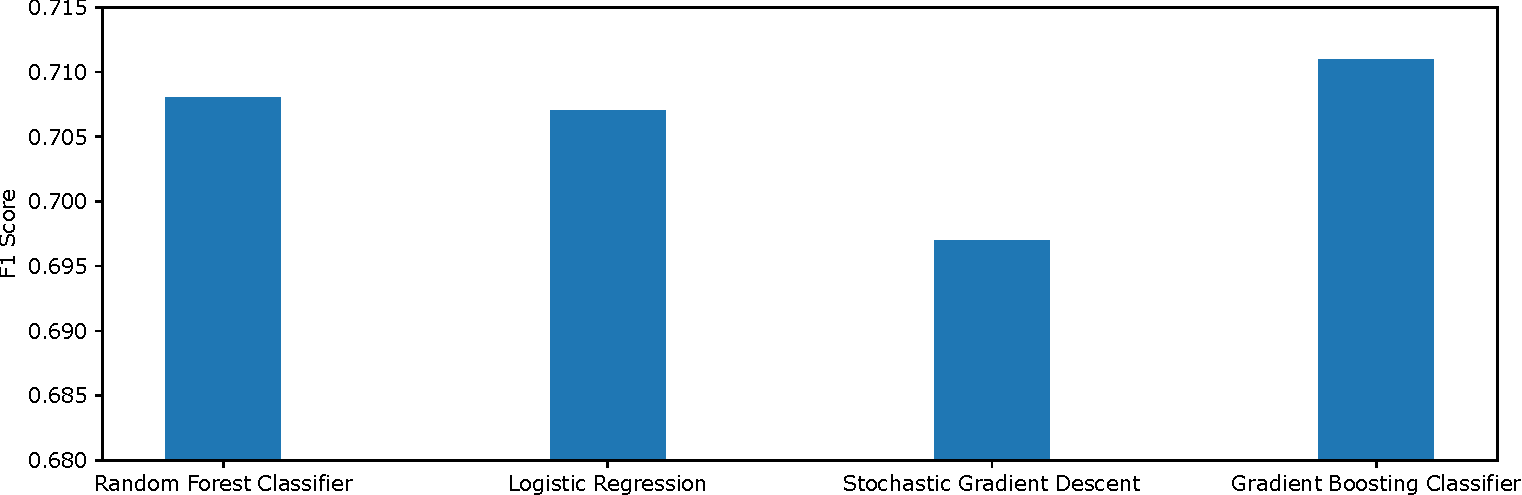
\includegraphics[width=1\textwidth]{images/models_f1_score.pdf}
	\caption{Model's best F1 score on the test data set}
	\label{fig:models_f1_score}
\end{figure}

The results are close across all the models, but the \textit{Gradient Boosting Classifier} had a slight edge over the remaining. 
%However, after a few tweaks with the  \textit{Gradient Boosting Classifier} baseline, it revealed a tendency to overfit by giving to much over \SI{60}{\percent} importance to a single feature. Thus, the \textit{Random Forest Classifier} was chosen to proceed the analysis. 
For that reason, the \textit{Gradient Boosting Classifier} was chosen to proceed the analysis.

\subsection{Known issues and risks}

The current approach is highly vulnerable to over-fitting, which is the main risk of the proposed model. This means the model may not be able to provide an accurate result for data it has never seen, specially when a medical encounter has details that were not available during training.

Also, the high dependency on a single variable may cause the model fail for observations where that variable is missing.

Furthermore, \textit{Gradient Boosting Classifier} is sensitive to outliers given the logic it uses to build its decision trees. This means that outliers on our current data set can have higher impact on the model performance. This problem is exacerbated by the random under-sampling used to balance the data, since outliers on the training set have a higher preponderance on the model.

The proposed model also fails to avoid discrimination, even though there are constraints in place to mitigate it. A higher volume of data may be useful to improve on this issue on a future iteration.

\newpage
\section{Model Deployment}
\subsection{Deployment specifications}


The predictive model was built taking into consideration its deployment and tried to be as generic as possible regarding the input data. This was achieved using the \texttt{sklearn} framework as it provides useful tools and boilerplate for this endeavour.
The model predictor is built within a \texttt{pipeline} that also contains \texttt{transformers}. More specifically, all variables from the provided dataset have its own \texttt{transformer} that either drops the variable or converts it into a valid input. Furthermore, \texttt{sklearn}'s \texttt{imputers} were also used to impute default values on variables that may be missing.
The combination of \texttt{transformers} and \texttt{imputers} allowed having a \texttt{pipeline} ready to handle a wide range of inputs, thus contributing to the overall application robustness.

The model deployment was also built to be as robust as possible. Even though the schema API has all the parameters marked as mandatory, the model deployment took into consideration edge cases that could crash the application. Thus, all the request fields can be missing and an output is still provided.

In order to keep track of the model performance and enable future deployments with up to date data, the application is integrated with a \texttt{postgres} database. This database contains a single table called \texttt{MedicalEncounter} that matches the raw data of the provided dataset according to table \ref{tab:dtypes}. Each variable on that table has its own column with a matching data type: either \texttt{Text}, \texttt{Integer}, or \texttt{Float}.
Furthermore, 3 extra columns were added: 

\begin{itemize}
    \item \texttt{proba}: a \texttt{Float} field to hold the model probability output for the current observation;
    \item \texttt{prediction}: a \texttt{Boolean} field to hold the actual model prediction based on the probability;
    
    \item \texttt{true\_label}: a \texttt{Boolean} field to store the actual expected outcome;
\end{itemize}


The database connection and queries are handle with \texttt{pewee}, a ORM (Object–relational mapping) library responsible for interpreting \texttt{python} instructions and data into the database equivalent, and vice-versa. It is used to connect with the database and build a representation model of the stored data.

The request data integrity is also assured using \texttt{pewee}.  Hence, why all expected fields are marked as either \texttt{text}, \texttt{float} or \texttt{boolean} with the advantage of \texttt{pewee} itself doing the type conversions. For instance, \texttt{pewee} recognizes the string \textit{"11"} as the number $11$ and still stores it as a \texttt{float}. When \texttt{pewee} fails to do the type conversion, the database will throw an error if the data type is invalid. Such exception is handled and modified into an error response message readable by the end user.

The web application was built using the python's library \texttt{flask} and provides two different endpoints as described in table \ref{tab:rest_api}. When an error occurs, for instance when there is data type mismatch as described above, both endpoints return an error response whose schema is detailed on algorithm \ref{alg:error_response}.


\begin{table}[htb]
\caption{REST API endpoints description}
\label{tab:rest_api}
\centering
\begin{tabularx}{1\textwidth}{llX}
\toprule
\multicolumn{1}{c}{\textsc{Method}} & \multicolumn{1}{l}{\textsc{Path}} & \multicolumn{1}{c}{\textsc{Description}} \\
\midrule
\texttt{POST} & \texttt{/predict} & \noindent\parbox[c]{\hsize}{\small Receives information regarding a single medical encounter, and outputs whether the patient should or should not be discharged. The request schema is detailed on algorithm \ref{alg:predict_request} and the response schema on algorithm \ref{alg:predict_response}. All unique prediction requests are stored in a database for future analysis.} \\
 & & \\
\texttt{POST} & \texttt{/update} & \noindent\parbox[c]{\hsize}{\small Receives one medical encounter identifier along with the real readmission information. The database should be updated accordingly for future reference. The request schema is detailed on algorithm \ref{alg:update_request} and the response schema on algorithm \ref{alg:update_response}.}\\
\bottomrule
\end{tabularx}
\end{table}

Naturally, errors may occur on both endpoints, and consequently there is an error response schema, detailed on algorithm \ref{alg:error_response}, used to handle those cases. The application has 4 different error types:

\begin{itemize}
    \item \texttt{INVALID\_REQUEST}: Triggered when a request does not match the expected format and it is not possible to infer the correct format.
    \item \texttt{DUPLICATED\_ADMISSION\_ID}: Triggered for duplicated \texttt{/predict} requests. This error message is not exposed outside the application of the application, since the app will recover from it and return the previous known prediction; 
    \item \texttt{DOES\_NOT\_EXIST}: Triggered when trying to update a medical encounter that does not exist in the database;
    \item \texttt{UNKNONW\_EXCEPTION}: General purpose error response. This error should never be triggered, since it is used for unpredicted runtime errors;
\end{itemize}

Finally, the whole application is deployed and published through \texttt{Heroku}. \texttt{Heroku} also provides the database resources used to collect the data throughout the application lifespan. 

\begin{figure}[!htb]
	
\begin{minipage}[t]{0.45\textwidth}
    \begin{algorithm}[H]
        \caption{\texttt{/predict} request schema}
        \label{alg:predict_request}
        \lstinputlisting{algorithms/predict_request.txt}
    \end{algorithm}
\end{minipage}%
\hfill
\begin{minipage}[t]{0.45\textwidth}
    \begin{algorithm}[H]
        \caption{\texttt{/predict} response schema}
        \label{alg:predict_response}
        \lstinputlisting{algorithms/predict_response.txt}
    \end{algorithm}
    \vspace{0.65em}
    \begin{algorithm}[H]
        \caption{\texttt{/update} request schema}
        \label{alg:update_request}
        \lstinputlisting{algorithms/update_request.txt}
    \end{algorithm}
    \vspace{0.65em}
    \begin{algorithm}[H]
        \caption{\texttt{/update} response schema}
        \label{alg:update_response}
        \lstinputlisting{algorithms/update_response.txt}
    \end{algorithm}
    \vspace{0.65em}
    \begin{algorithm}[H]
        \caption{Error response schema}
        \label{alg:error_response}
        \lstinputlisting{algorithms/error_response.txt}
    \end{algorithm}
\end{minipage}


	\caption{Endpoints' request, response and error schema}
	\label{fig:endpoint_requests_schema}
\end{figure}




% All values are marked as required in the request, which is not going to be true, thus:
% Robustez foi um dos principais objectivos

%Inês Mendes (instructor - devops)  7 days ago
%I tend to do all of my transformation through custom transformers, so my pipeline can take raw data, but I don't see why the second option wouldn't work
%https://github.com/LDSSA/heroku-model-deploy#put-your-custom-code-in-a-package

\subsection{Known issues and risks}

Event though robustness was one of the key factors in the application deployment, there are a few details worth noting. First of all, the application is not fault tolerant regarding the request's field names. This means, that a typo on the request is interpreted as a missing field. Missing fields, however, will not impact the application's health, but may skew the model correctness.

Furthermore, the application discards duplicated medical encounters and keeps only the first occurrence. This may be an issue if the first request of a given encounter has missing information that is available on a second request.

Also, the application is \SI{100}{\percent} dependent on the \texttt{Heroku} service provider availability. If for any reason, \texttt{Heroku}'s services are down or compromised, the REST API follows suit. Furthemore, \texttt{Heroku} imposes limitations on the application usage:

\begin{itemize}
    \item Maximum \SI{10000}{} unique records on the database;
    \item Maximum of \SI{4500}{requests}  per hour;
    \item The logging availability is limited to the last \SI{1500}{lines}.
\end{itemize}

Regarding security, the data provided to the REST API is stored in clear text on the data base, including sensitive patient data. This means, that an attacker with elevated access to our system could download these information.
Once more, the app relies entirely on \texttt{Heroku} security to handle access authorization. However, this also means that a breach on their systems could also comprise the data stored by the REST API.

Finally, \texttt{Heroku} sets its applications to sleep if they receive no traffic within \SI{1}{\hour}. When that happens, it is expected for the first requests to suffer a small delay. Nonetheless, all requests should perform as expected after the application has wakened.


\newpage
\section{Annexes}
\subsection{Dataset technical analysis}
\label{subsection:tech_analysis}

\begin{table}[H]
\caption{Dataset variables' types before and after pre-processing }
\label{tab:dtypes}
\centering
\begin{tabularx}{1\textwidth}{XYY}
\toprule
\textsc{Variable} &        \textsc{Original Type} & \textsc{Pre-processed Type}\\
\midrule
\admissionId                &    \texttt{int64} &     \texttt{int64} \\
\patientId                  &    \texttt{int64} &     \texttt{int64} \\
\race                        &   \texttt{object} &  \texttt{category} \\
\gender                      &   \texttt{object} &  \texttt{category} \\
\age                         &   \texttt{object} &     \texttt{Int64} \\
\weight                      &   \texttt{object} &     \texttt{Int64} \\
\admissionTypeCode         &  \texttt{float64} &  \texttt{category} \\
\dischargeDispositionCode  &  \texttt{float64} &  \texttt{category} \\
\admissionSourceCode       &    \texttt{int64} &  \texttt{category} \\
\timeInHospital            &    \texttt{int64} &     \texttt{int64} \\
\payerCode                  &   \texttt{object} &  \texttt{category} \\
\medicalSpecialty           &   \texttt{object} &  \texttt{category} \\
\hasProsthesis              &     \texttt{bool} &      \texttt{bool} \\
\completeVaccinationStatus &   \texttt{object} &  \texttt{category} \\
\numLabProcedures          &  \texttt{float64} &     \texttt{Int64} \\
\numProcedures              &    \texttt{int64} &     \texttt{int64} \\
\numMedications             &  \texttt{float64} &     \texttt{Int64} \\
\numberOutpatient           &    \texttt{int64} &     \texttt{int64} \\
\numberEmergency            &    \texttt{int64} &     \texttt{int64} \\
\numberInpatient            &    \texttt{int64} &     \texttt{int64} \\
\diagOne                      &   \texttt{object} &  \texttt{category} \\
\diagTwo                      &   \texttt{object} &  \texttt{category} \\
\diagThree                      &   \texttt{object} &  \texttt{category} \\
\numberDiagnoses            &    \texttt{int64} &     \texttt{int64} \\
\bloodType                  &   \texttt{object} &  \texttt{category} \\
\hemoglobinLevel            &  \texttt{float64} &   \texttt{float64} \\
\bloodTransfusion           &     \texttt{bool} &      \texttt{bool} \\
\maxGluSerum               &   \texttt{object} &  \texttt{category} \\
\AOneCresult                   &   \texttt{object} &  \texttt{category} \\
\diuretics                   &   \texttt{object} &      \texttt{bool} \\
\insulin                     &   \texttt{object} &      \texttt{bool} \\
\change                      &   \texttt{object} &      \texttt{bool} \\
\diabetesMed                 &   \texttt{object} &      \texttt{bool} \\
\readmitted                  &   \texttt{object} &      \texttt{bool} \\
\bottomrule
\end{tabularx}
\end{table}

\begin{table}[H]
\caption{Numerical variables description after pre-processing }
\label{tab:dataset_describe}
\centering
\begin{tabularx}{\textwidth}{Xcccccccc}
\toprule
\textsc{Variable} &  \textsc{count} &   \textsc{mean} &    \textsc{std} & \textsc{min} & \textsc{\SI{25}{\percent}} & \textsc{\SI{50}{\percent}} &  \textsc{\SI{75}{\percent}} &  \textsc{max} \\
\midrule
\age                &  79076 &  60.96 &  15.97 &   0 &  50 &  60 &   70 &   90 \\
\weight             &   2499 &  73.67 &  26.23 &   0 &  50 &  75 &  100 &  200 \\
\timeInHospital   &  81412 &   4.40 &   2.98 &   1 &   2 &   4 &    6 &   14 \\
\numLabProcedures &  79919 &  43.07 &  19.63 &   1 &  32 &  44 &   57 &  132 \\
\numProcedures     &  81412 &   1.34 &   1.71 &   0 &   0 &   1 &    2 &    6 \\
\numMedications    &  78734 &  16.02 &   8.11 &   1 &  10 &  15 &   20 &   81 \\
\numberOutpatient  &  81412 &   0.37 &   1.28 &   0 &   0 &   0 &    0 &   42 \\
\numberEmergency   &  81412 &   0.20 &   0.88 &   0 &   0 &   0 &    0 &   64 \\
\numberInpatient   &  81412 &   0.64 &   1.27 &   0 &   0 &   0 &    1 &   21 \\
\numberDiagnoses   &  81412 &   7.42 &   1.93 &   1 &   6 &   8 &    9 &   16 \\
\hemoglobinLevel   &  81412 &  14.19 &   1.06 &  10 &  13 &  14 &   15 &   19 \\
\bottomrule
\end{tabularx}
\end{table}

%\subsection{Business questions technical support}
\label{subsection:business_tech_analysis}

\newgeometry{bottom=0.3in, top=0.3in}
\begin{landscape}

\label{sec:business_questions_tech}

\thispagestyle{empty}
\begin{table}[H]
\caption{Detailed per-specialty discrimination analysis on the new collected data. All values are normalized to the overall medical specialty readmission occurrence on the last column. Values above the \SI{25}{\percent} threshold are marked in \textbf{bold}, values below the threshold are \underline{underlined}. Dashes mean there were no occurrences for that class, whilst zeros mean there no re-admissions for that class.}
\label{tab:discrimination_analysis}
\centering
\footnotesize
\begin{tabular}{l||ccccccccccc||cc||ccccc||cc||c}
\toprule
\multicolumn{1}{c||}{\textsc{\small Medical}} & \multicolumn{11}{c||}{\textsc{\small Age}} & \multicolumn{2}{c||}{\textsc{\small Gender}} & \multicolumn{5}{c||}{\textsc{\small Race}} & \multicolumn{2}{c||}{\textsc{\small Insured}} & \textsc{\small Spec.} \\
\multicolumn{1}{c||}{\textsc{\small Specialty}} &     0 & 10 & 20 & 30 & 40 & 50 & 60 & 70 & 80 & 90 & NA &  F &  M &  asian &  Black &  Hisp. &  Other &  White &  Yes &  No &  \textsc{\small Rate}\\
\midrule
Endocrinology          &         - &              - &    \textbf{11.00} &                 - &          \tiny{0} &          \tiny{0} &          \tiny{0} &          \tiny{0} &                 - &                 - &                 - &  \textbf{2.20} &          \tiny{0} &              - &          \tiny{0} &                 - &                 - &     \textbf{1.57} &                 - &        1.00 &    0.09 \\
Others                 &  \tiny{0} &       \tiny{0} &     \textbf{1.52} &     \textbf{1.28} &              0.84 &              0.97 &              1.02 &              0.96 &              1.04 &     \textbf{1.50} &              0.77 &           1.04 &              0.96 &       \tiny{0} &              0.99 &  \underline{0.71} &  \underline{0.31} &              1.05 &              0.80 &        1.01 &    0.13 \\
Family/GeneralPractice &         - &       \tiny{0} &              0.90 &  \underline{0.56} &              1.14 &              0.76 &              1.02 &              1.08 &              1.19 &  \underline{0.50} &     \textbf{1.30} &           1.01 &              0.99 &  \textbf{1.35} &              1.24 &          \tiny{0} &  \underline{0.48} &              1.01 &              0.87 &        1.01 &    0.15 \\
Radiology              &         - &              - &                 - &                 - &     \textbf{2.56} &     \textbf{1.33} &  \underline{0.67} &     \textbf{1.38} &          \tiny{0} &          \tiny{0} &          \tiny{0} &  \textbf{1.32} &  \underline{0.72} &              - &     \textbf{2.05} &                 - &          \tiny{0} &              0.92 &              1.14 &        0.99 &    0.10 \\
Orthopedics            &         - &              - &          \tiny{0} &          \tiny{0} &     \textbf{2.08} &  \underline{0.74} &              0.94 &              0.97 &     \textbf{1.40} &     \textbf{6.78} &          \tiny{0} &  \textbf{1.33} &  \underline{0.41} &              - &              0.88 &          \tiny{0} &                 - &              0.94 &          \tiny{0} &        1.03 &    0.07 \\
InternalMedicine       &         - &       \tiny{0} &  \underline{0.54} &              0.96 &              0.86 &  \underline{0.70} &              1.15 &              1.07 &              1.16 &  \underline{0.34} &              1.22 &           0.95 &              1.07 &  \textbf{1.56} &              0.83 &     \textbf{1.30} &     \textbf{1.34} &              1.07 &  \underline{0.23} &        1.02 &    0.14 \\
Emergency/Trauma       &         - &       \tiny{0} &              1.23 &              1.13 &     \textbf{1.35} &  \underline{0.62} &     \textbf{1.29} &              1.02 &              0.84 &              0.89 &  \underline{0.70} &           0.89 &              1.14 &           1.23 &  \underline{0.70} &  \underline{0.74} &              0.82 &              1.05 &              0.82 &        1.04 &    0.14 \\
Pulmonology            &         - &              - &                 - &     \textbf{4.20} &          \tiny{0} &  \underline{0.65} &  \underline{0.42} &     \textbf{1.46} &          \tiny{0} &     \textbf{4.20} &     \textbf{2.80} &           0.84 &              1.15 &  \textbf{4.20} &              1.10 &          \tiny{0} &          \tiny{0} &  \underline{0.66} &          \tiny{0} &        1.05 &    0.12 \\
Gynecology/Obstetrics  &         - &  \textbf{5.83} &  \underline{0.73} &  \underline{0.65} &  \underline{0.73} &     \textbf{1.67} &          \tiny{0} &          \tiny{0} &          \tiny{0} &    \textbf{11.67} &                 - &           1.00 &                 - &       \tiny{0} &     \textbf{2.75} &          \tiny{0} &          \tiny{0} &  \underline{0.53} &          \tiny{0} &        1.01 &    0.09 \\
Surgery                &         - &  \textbf{4.05} &     \textbf{3.24} &  \underline{0.37} &     \textbf{1.42} &              1.18 &              0.83 &              1.06 &              0.90 &          \tiny{0} &  \underline{0.40} &           0.93 &              1.06 &       \tiny{0} &              0.80 &              1.16 &     \textbf{1.35} &              1.02 &              1.19 &        0.99 &    0.12 \\
Cardiology             &         - &              - &     \textbf{9.94} &     \textbf{1.99} &              0.95 &              0.82 &  \underline{0.54} &     \textbf{1.35} &     \textbf{1.40} &          \tiny{0} &  \underline{0.66} &           0.88 &              1.10 &  \textbf{9.94} &     \textbf{1.36} &          \tiny{0} &  \underline{0.66} &              0.93 &  \underline{0.62} &        1.01 &    0.10 \\
Pediatrics             &  \tiny{0} &  \textbf{1.76} &                 - &                 - &          \tiny{0} &          \tiny{0} &          \tiny{0} &          \tiny{0} &                 - &                 - &          \tiny{0} &  \textbf{1.69} &          \tiny{0} &       \tiny{0} &     \textbf{4.89} &                 - &                 - &          \tiny{0} &          \tiny{0} &        1.02 &    0.02 \\
Nephrology             &         - &              - &     \textbf{5.30} &              0.76 &  \underline{0.48} &              1.16 &              0.78 &              1.15 &     \textbf{2.12} &                 - &          \tiny{0} &           0.76 &              1.21 &              - &              0.98 &                 - &          \tiny{0} &              1.06 &          \tiny{0} &        1.02 &    0.19 \\
PhysicalMedicine       &         - &              - &                 - &          \tiny{0} &          \tiny{0} &          \tiny{0} &  \underline{0.72} &              1.21 &     \textbf{1.44} &                 - &                 - &           0.88 &              1.15 &              - &          \tiny{0} &          \tiny{0} &     \textbf{5.75} &              1.06 &                 - &        1.00 &    0.17 \\
Gastroenterology       &         - &              - &                 - &          \tiny{0} &          \tiny{0} &              0.85 &              1.24 &     \textbf{1.87} &              1.17 &          \tiny{0} &          \tiny{0} &           1.00 &              1.00 &              - &     \textbf{1.56} &                 - &                 - &              0.93 &                 - &        1.00 &    0.11 \\
Hematology             &         - &              - &                 - &                 - &                 - &          \tiny{0} &          \tiny{0} &     \textbf{1.28} &     \textbf{2.56} &                 - &                 - &           1.02 &              0.96 &              - &                 - &                 - &                 - &              1.00 &          \tiny{0} &        1.05 &    0.26 \\
Psychiatry             &         - &  \textbf{1.73} &  \underline{0.74} &          \tiny{0} &              0.92 &              1.20 &              1.22 &     \textbf{1.60} &  \underline{0.74} &                 - &          \tiny{0} &           0.92 &              1.11 &              - &  \underline{0.60} &                 - &          \tiny{0} &              1.16 &          \tiny{0} &        1.07 &    0.19 \\
Neurology              &         - &              - &                 - &                 - &                 - &                 - &                 - &                 - &                 - &                 - &                 - &              - &                 - &              - &                 - &                 - &                 - &                 - &                 - &           - &    0.00 \\
Urology                &         - &              - &                 - &          \tiny{0} &          \tiny{0} &     \textbf{2.21} &  \underline{0.55} &     \textbf{2.15} &          \tiny{0} &                 - &          \tiny{0} &  \textbf{1.28} &              0.90 &              - &     \textbf{2.70} &          \tiny{0} &                 - &              0.81 &          \tiny{0} &        1.01 &    0.08 \\
Oncology               &         - &              - &                 - &     \textbf{3.40} &     \textbf{1.70} &              0.97 &  \underline{0.57} &  \underline{0.68} &     \textbf{1.36} &                 - &          \tiny{0} &           1.00 &              1.00 &              - &              0.97 &                 - &          \tiny{0} &              1.09 &                 - &        1.00 &    0.29 \\
InfectiousDiseases     &         - &              - &                 - &     \textbf{2.00} &                 - &                 - &          \tiny{0} &                 - &              1.00 &                 - &                 - &  \textbf{1.33} &          \tiny{0} &              - &              1.00 &                 - &                 - &              1.00 &                 - &        1.00 &    0.50 \\
Podiatry               &         - &              - &                 - &                 - &                 - &                 - &                 - &                 - &                 - &                 - &                 - &              - &                 - &              - &                 - &                 - &                 - &                 - &                 - &           - &    0.00 \\
Anesthesiology         &         - &              - &                 - &                 - &                 - &                 - &                 - &                 - &                 - &                 - &                 - &              - &                 - &              - &                 - &                 - &                 - &                 - &                 - &           - &    0.00 \\
Ophthalmology          &         - &              - &                 - &                 - &                 - &                 - &                 - &                 - &                 - &                 - &                 - &              - &                 - &              - &                 - &                 - &                 - &                 - &                 - &           - &    0.00 \\
\bottomrule
\end{tabular}
\end{table}

\end{landscape}
\restoregeometry



\begin{figure}[!htb]
	\centering
	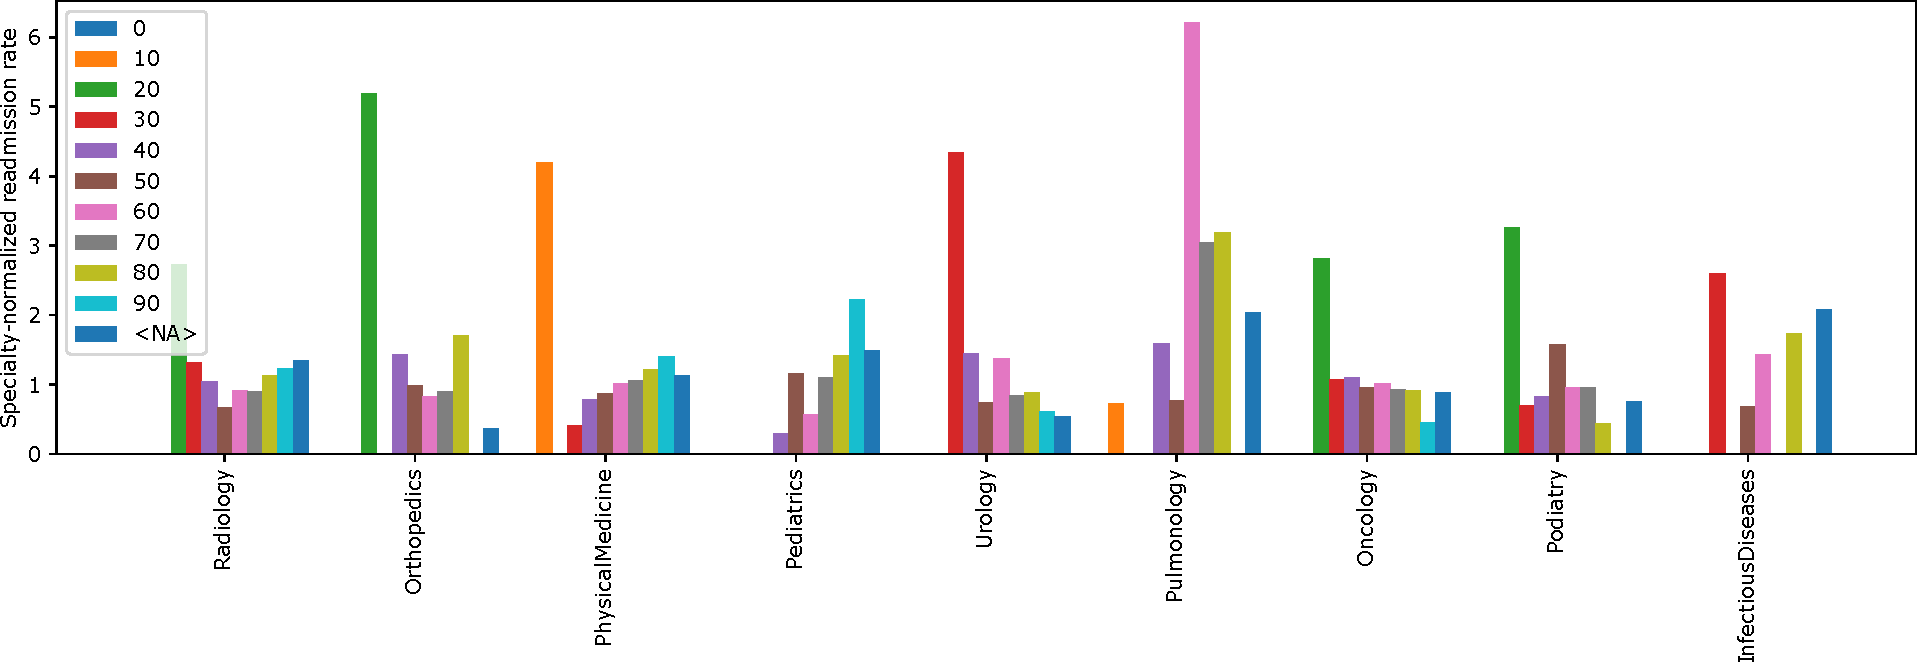
\includegraphics[width=1\textwidth]{images/descrimination_histogram_age.pdf}
	\caption{Age discrimination analysis per medical specialty}
	\label{fig:discrimination_histogram_age}
\end{figure}

\begin{figure}[!htb]
	\centering
	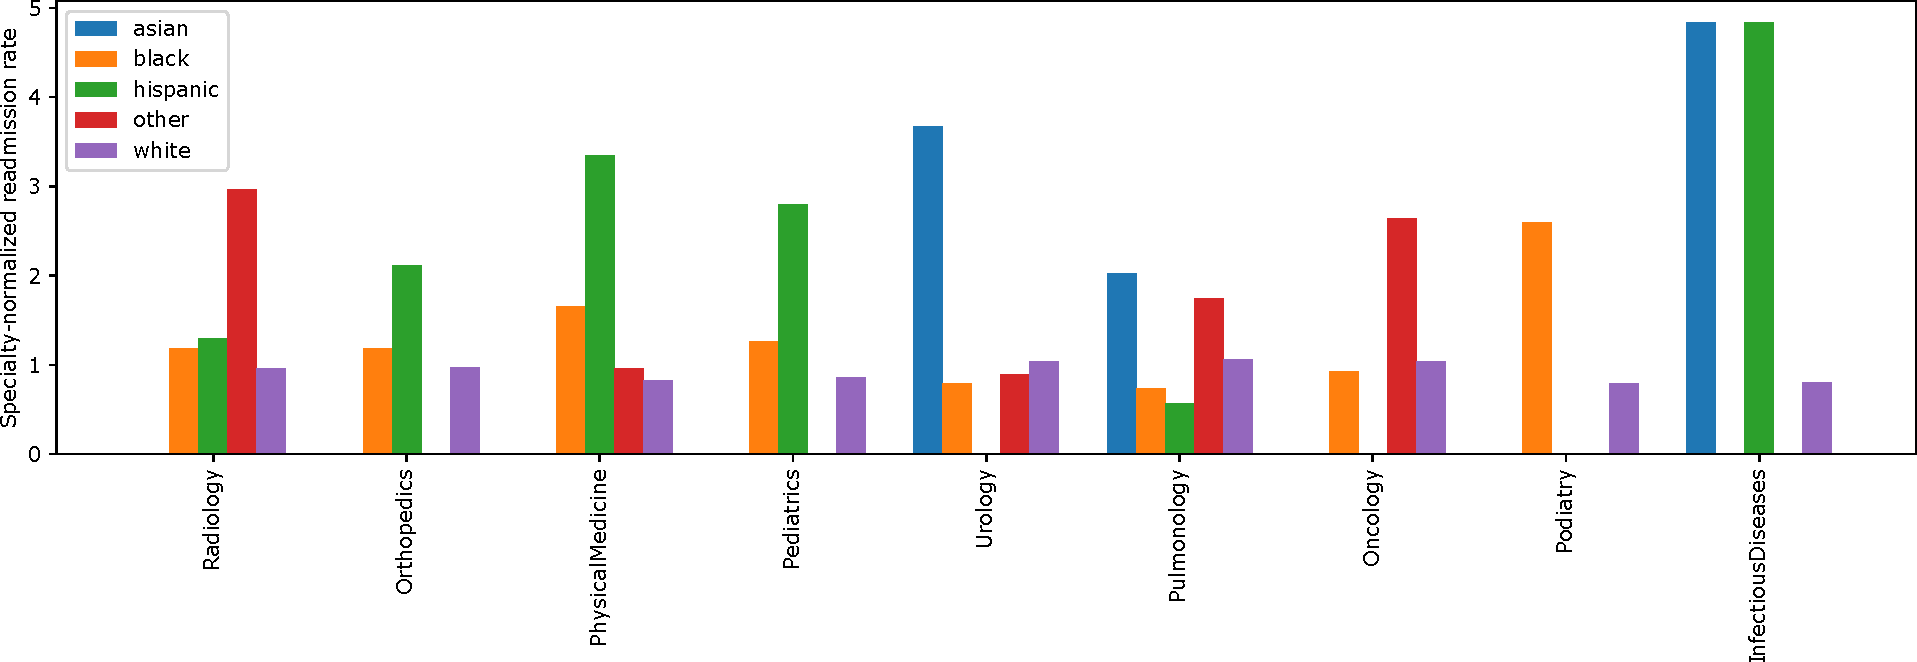
\includegraphics[width=1\textwidth]{images/descrimination_histogram_race.pdf}
	\caption{Race discrimination analysis per medical specialty}
	\label{fig:discrimination_histogram_race}
\end{figure}

\begin{figure}[!htb]
	\centering
	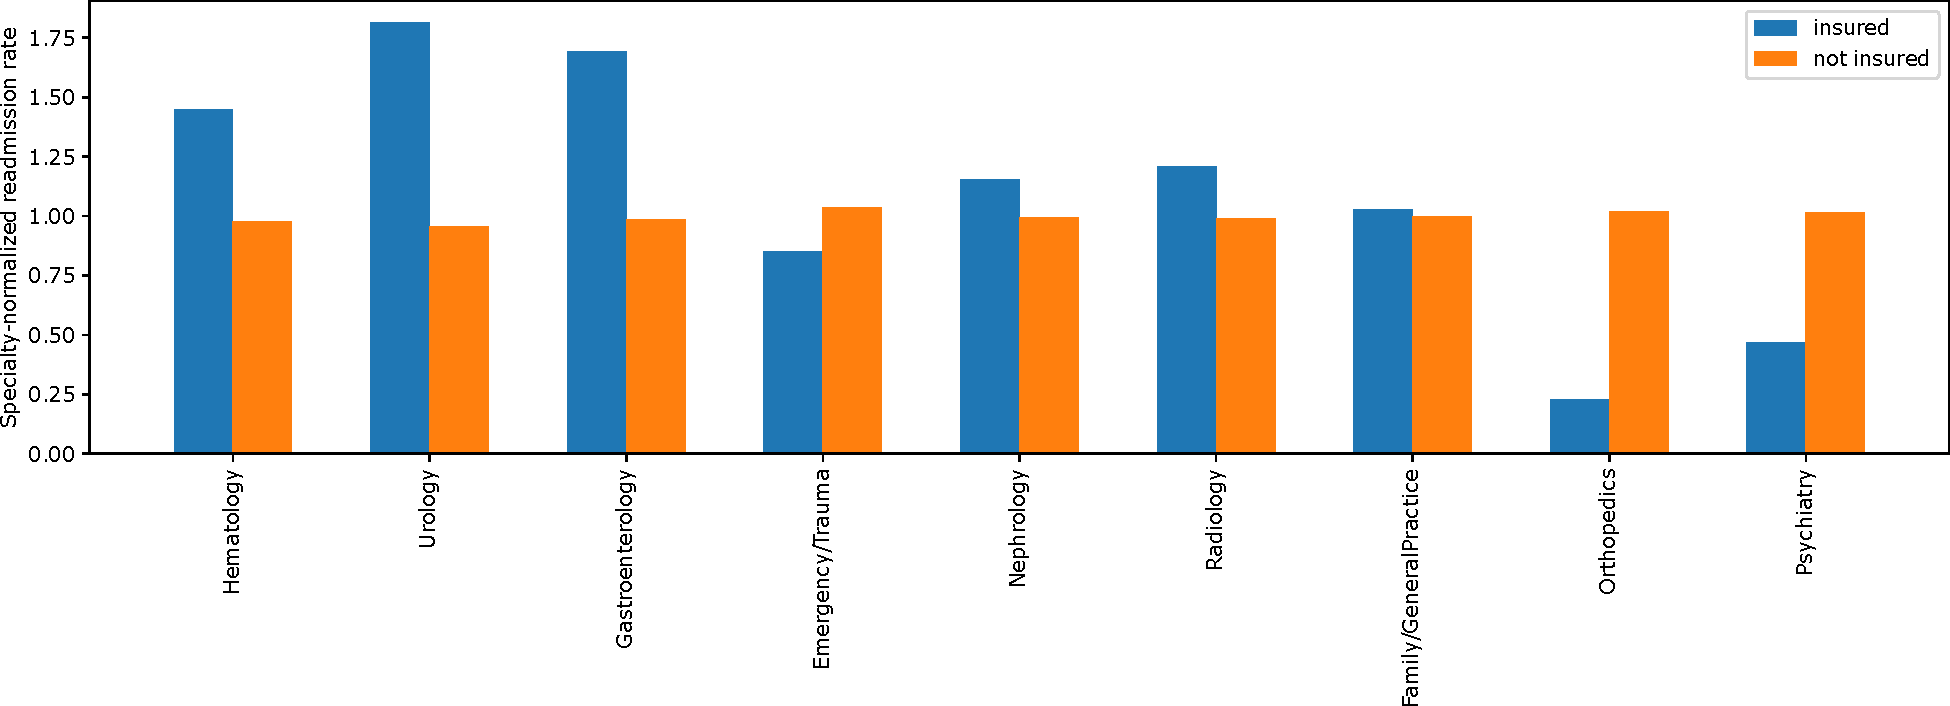
\includegraphics[width=1\textwidth]{images/descrimination_histogram_is_insured.pdf}
	\caption{Insurance status discrimination analysis per medical specialty}
	\label{fig:discrimination_histogram_is_insured}
\end{figure}

\newpage
\subsection{Model technical analysis}
\label{sec:model_technical_analysis}


\begin{table}[htb]
\centering
\caption{Predictive model's best F1 score on the test data set}
\label{tab:models_f1_score}
\begin{tabularx}{0.6\textwidth}{Yc}
\toprule
\textsc{Model} & \textsc{F1 Score} \\
\midrule
\texttt{Random Forest Classifier}               & 0.708 \\
\texttt{Logistic Regression}                    & 0.707 \\
\texttt{Stochastic Gradient Descent}            & 0.697 \\
\texttt{Gradient Boosting Classifier}           & \textbf{0.711} \\
\bottomrule
\end{tabularx}
\end{table}


% Please add the following required packages to your document preamble:
% \usepackage{multirow}
\begin{table}[htb]
\caption{Predictive model's threshold that maximizes precision but keeping recall higher than \SI{50}{\percent} both on the training and the test data set, using the default hyper-parameters}
\label{tab:models_threshold}
\begin{tabularx}{\textwidth}{lYcccc}
\toprule
                       & \textsc{Model} & \textsc{Threshold} & \textsc{Precision} & \textsc{Recal} & \textsc{F1} \\
\midrule
\multirow{4}{*}{\textsc{Train}} & \texttt{Random Forest Classifier}      & 0.85      & \textbf{1.000}                 & \textbf{0.520}             & \textbf{0.685}         \\
                       & \texttt{Logistic Regression}                    & 0.64      & 0.835                 & 0.502             & 0.627         \\
                       & \texttt{Stochastic Gradient Descent}            & 0.64      & 0.821                 & 0.509             & 0.629         \\
                       & \texttt{Gradient Boosting Classifier}           & 0.65      & 0.832                 & 0.507             & 0.630         \\
\midrule
\multirow{4}{*}{\textsc{Test}}  & \texttt{Random Forest Classifier}      & 0.60      & 0.794                 & 0.500             & 0.614         \\
                       & \texttt{Logistic Regression}                    & 0.61      & 0.797                 & 0.500             & 0.614         \\
                       & \texttt{Stochastic Gradient Descent}            & 0.61      & 0.791                 & \textbf{0.510}             & \textbf{0.620}         \\
                       & \texttt{Gradient Boosting Classifier}           & 0.62      & \textbf{0.798}                 & 0.501             & 0.616    \\
\bottomrule
\end{tabularx}
\end{table}


%\begin{figure}[!htb]
%	\centering
%	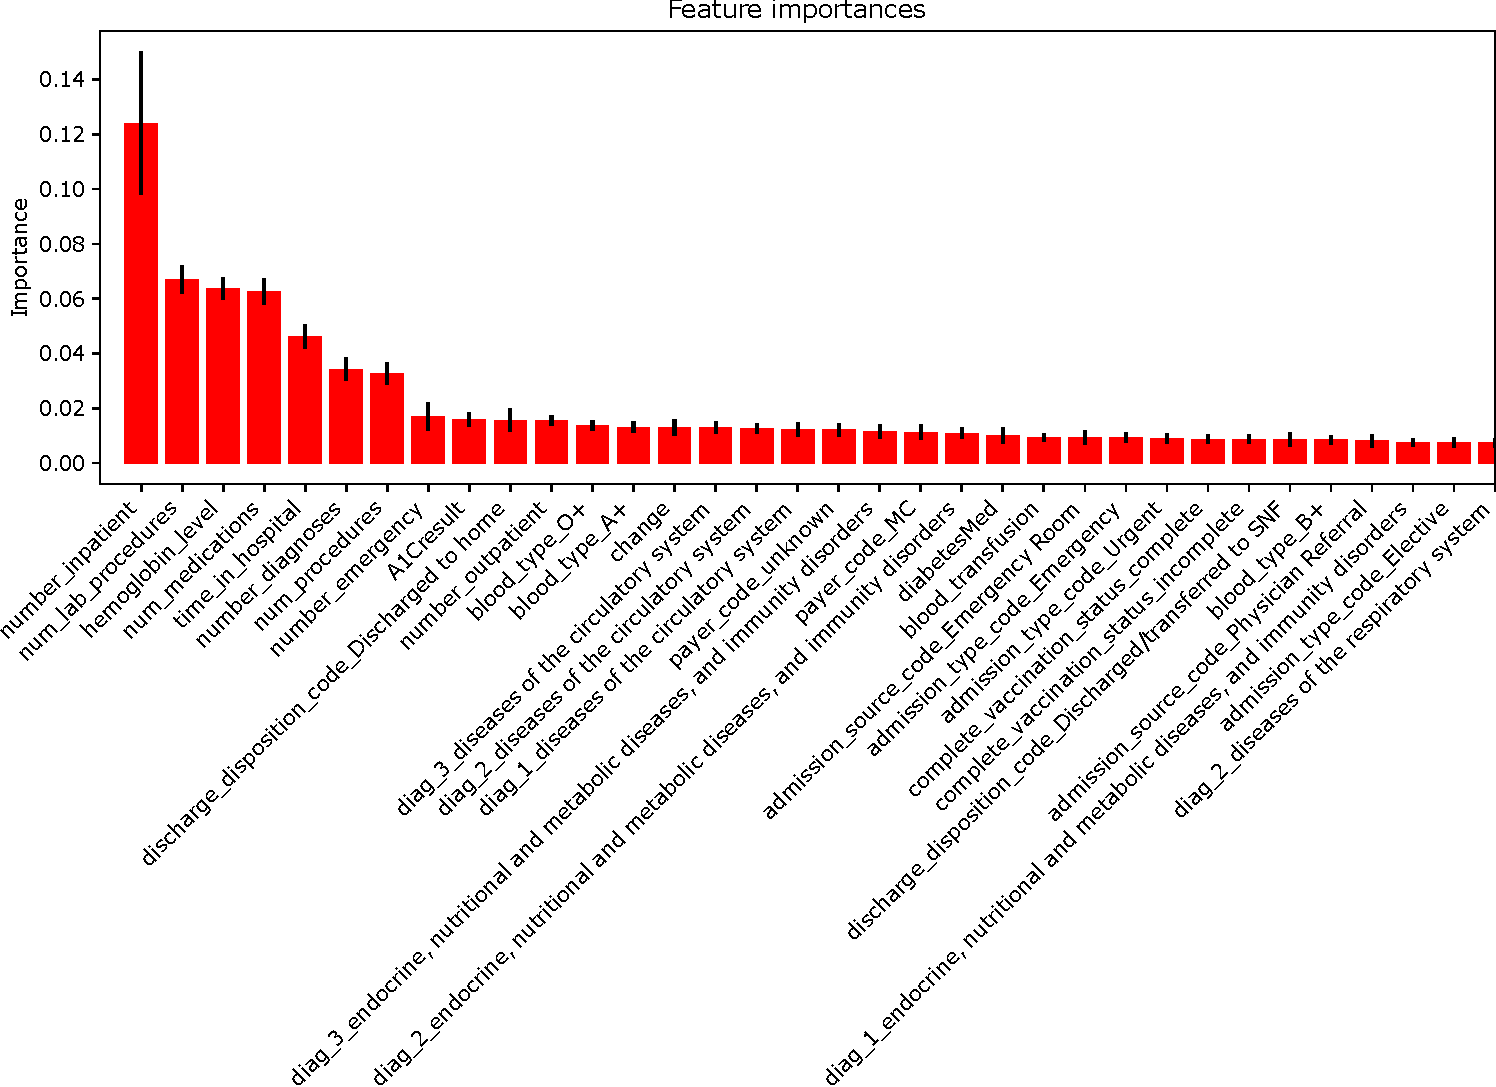
\includegraphics[width=1\textwidth]{images/feature_importance_rfc_overfitted.pdf}
%	\caption{Over-fitted \textit{Random Forest Classifier}, with infinite depth, feature importance}
%	\label{fig:feature_importance}
%\end{figure}

\vspace{2em}
\begin{figure}[!htb]
	\centering
	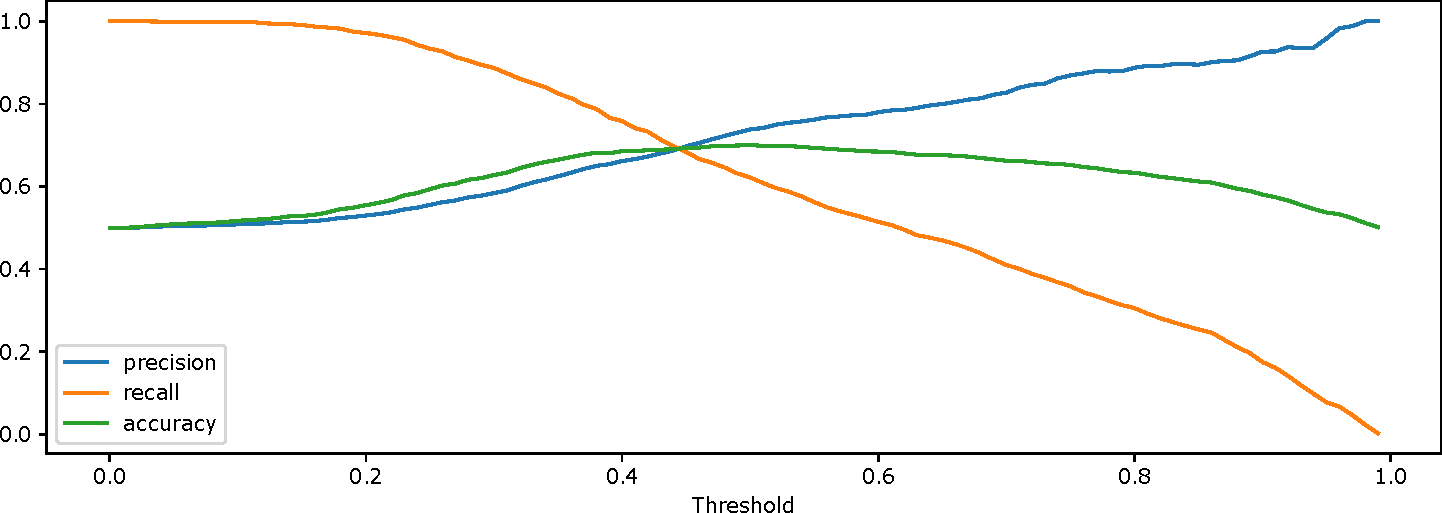
\includegraphics[width=1\textwidth]{images/precision_recall_evolution.pdf}
	\caption{Precision, recall, and accuracy evolution as the threshold increases}
	\label{fig:precision_recall_evolution}
\end{figure}

\begin{table}[htb]
\caption{\textit{Gradient Boosting Classifier} detailed feature importance graphically displayed on figure \ref{fig:feature_importance}}
\label{tab:model_feature_importance}
\begin{tabularx}{\textwidth}{Pc}
\toprule
\textsc{Feature Name} & \textsc{Importance} \\
\midrule
\texttt{\small number\_inpatient} & \SI{30.87}{\percent} \\
\texttt{\small number\_outpatient} & \SI{8.55}{\percent} \\
\texttt{\small number\_emergency} & \SI{8.45}{\percent} \\
\texttt{\small number\_diagnoses} & \SI{6.79}{\percent} \\
\texttt{\small discharge\_disposition\_code\_Expired} & \SI{6.62}{\percent} \\
\texttt{\small discharge\_disposition\_code\_Discharged to home} & \SI{6.55}{\percent} \\
\texttt{\small time\_in\_hospital} & \SI{4.90}{\percent} \\
\texttt{\small discharge\_disposition\_code\_Discharged/transferred to rehab fac} & \SI{4.80}{\percent} \\
\texttt{\small discharge\_disposition\_code\_Discharged/transferred to SNF} & \SI{3.84}{\percent} \\
\texttt{\small num\_medications} & \SI{3.53}{\percent} \\
\texttt{\small admission\_source\_code\_Emergency Room} & \SI{3.14}{\percent} \\
\texttt{\small num\_lab\_procedures} & \SI{1.39}{\percent} \\
\texttt{\small diag\_1\_diseases of the musculoskeletal system} & \SI{1.37}{\percent} \\
\texttt{\small diag\_3\_diseases of the genitourinary system} & \SI{1.30}{\percent} \\
\texttt{\small diag\_1\_symptoms, signs, and ill-defined conditions} & \SI{0.99}{\percent} \\
\texttt{\small payer\_code\_MC} & \SI{0.80}{\percent} \\
\texttt{\small payer\_code\_BC} & \SI{0.61}{\percent} \\
\texttt{\small diag\_2\_diseases of the skin and subcutaneous tissue} & \SI{0.57}{\percent} \\
\texttt{\small admission\_source\_code\_Clinic Referral} & \SI{0.44}{\percent} \\
\texttt{\small admission\_source\_code\_Physician Referral} & \SI{0.43}{\percent} \\
\texttt{\small A1Cresult} & \SI{0.41}{\percent} \\
\texttt{\small discharge\_disposition\_code\_Discharged/transferred to home} & \SI{0.32}{\percent} \\
\texttt{\small discharge\_disposition\_code\_Discharged/transferred to another} & \SI{0.27}{\percent} \\
\texttt{\small num\_procedures} & \SI{0.26}{\percent} \\
\texttt{\small hemoglobin\_level} & \SI{0.25}{\percent} \\
\texttt{\small diag\_1\_external causes of injury} & \SI{0.21}{\percent} \\
\texttt{\small diag\_3\_endocrine, nutritional and metabolic diseases} & \SI{0.16}{\percent} \\
\texttt{\small diag\_2\_complications of pregnancy, childbirth} & \SI{0.16}{\percent} \\
\texttt{\small diag\_2\_infectious and parasitic diseases} & \SI{0.14}{\percent} \\
\texttt{\small discharge\_disposition\_code\_Hospice / medical facility} & \SI{0.12}{\percent} \\
\texttt{\small admission\_type\_code\_Urgent} & \SI{0.12}{\percent} \\
\texttt{\small admission\_type\_code\_Emergency} & \SI{0.11}{\percent} \\
\texttt{\small admission\_source\_code\_Transfer from a hospital} & \SI{0.10}{\percent} \\
\bottomrule
\end{tabularx}
\end{table}

\begin{figure}[htb]
\centering
\begin{subfigure}{0.49\textwidth}
    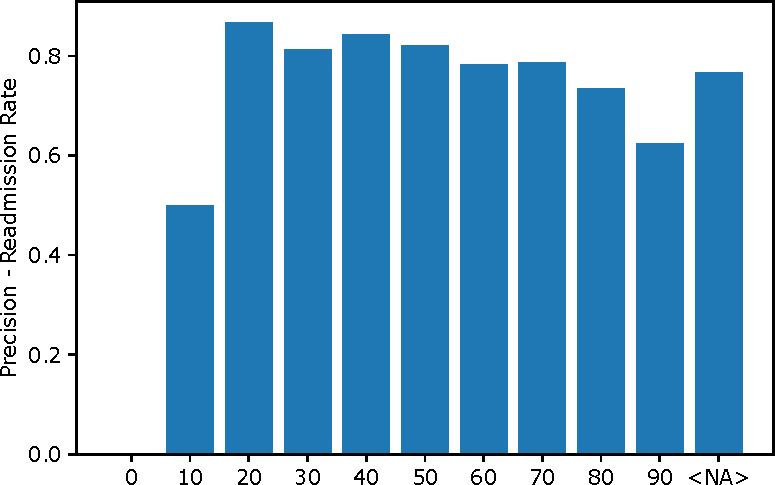
\includegraphics[width=\textwidth]{images/discrimination_requirement_age.pdf}
    \caption{Age}
    \label{fig:discrim_req_sensitive_age}
\end{subfigure}
\hfill
\begin{subfigure}{0.49\textwidth}
    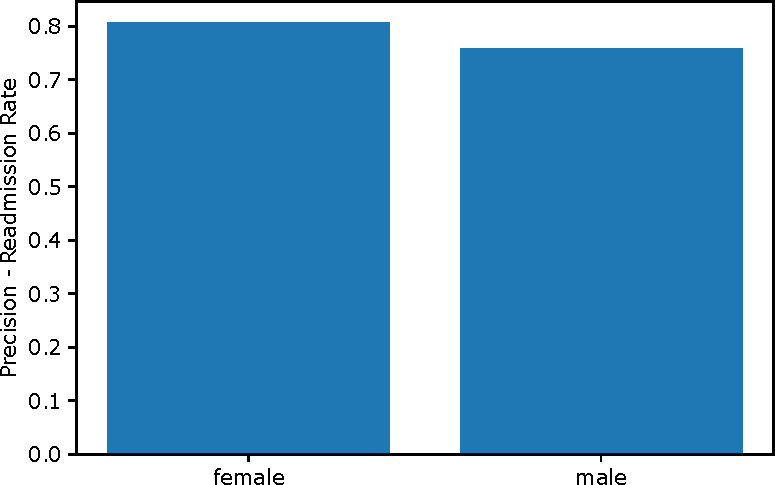
\includegraphics[width=\textwidth]{images/discrimination_requirement_gender.pdf}
    \caption{Gender}
    \label{fig:discrim_req_sensitive_gender}
\end{subfigure}
\begin{subfigure}{0.49\textwidth}
    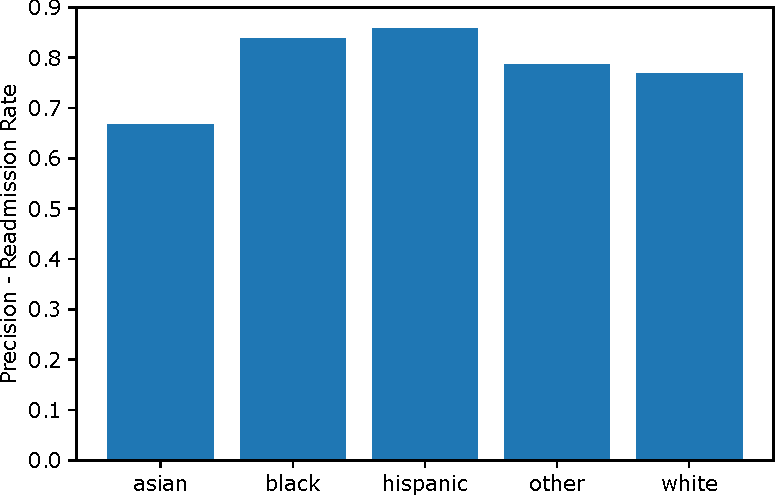
\includegraphics[width=\textwidth]{images/discrimination_requirement_race.pdf}
    \caption{Race}
    \label{fig:discrim_req_sensitive_race}
\end{subfigure}
\hfill
\begin{subfigure}{0.49\textwidth}
    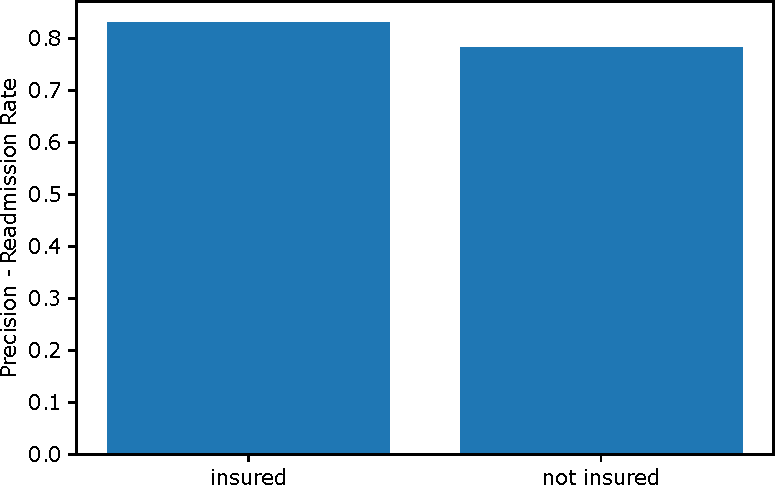
\includegraphics[width=\textwidth]{images/discrimination_requirement_is_insured.pdf}
    \caption{Insurance status}
    \label{fig:discrim_req_sensitive_is_insured}
\end{subfigure}
\caption{Model readmission rate for sensitive sub-groups}
\label{fig:discrim_req_sensitive}
\end{figure}

\begin{figure}[!htb]
	\centering
	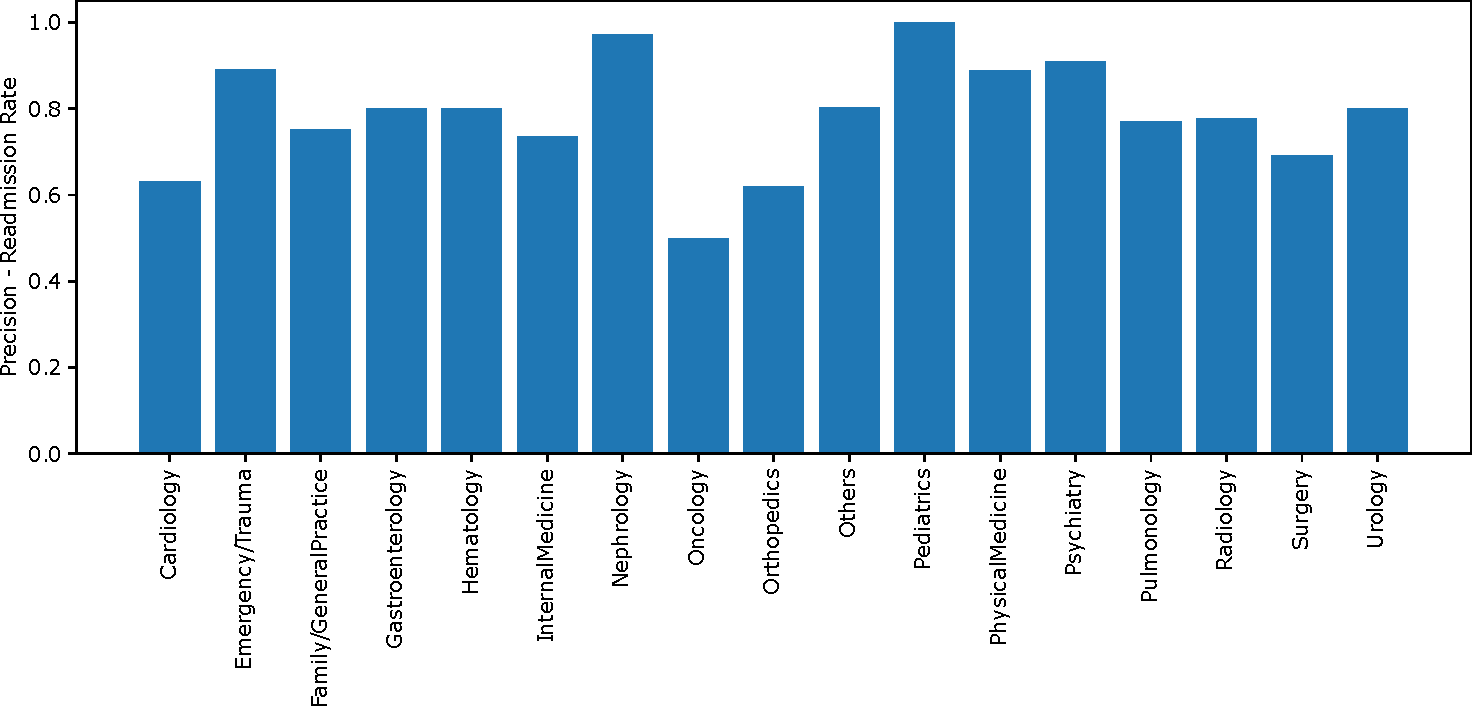
\includegraphics[width=1\textwidth]{images/discrimination_requirement_medical_specialty.pdf}
	\caption{Model readmission rate for medical specialties}
	\label{fig:discrim_req_medical_specialty}
\end{figure}








\end{document}
